\documentclass[]{article}
\usepackage[margin=1in]{geometry}
\usepackage{amsthm}
\usepackage{mathtools}
\usepackage{amsfonts}
\usepackage{multicol}
\usepackage{tikz}
\usepackage{eurosym}
\usepackage{algorithm}
\usepackage{algorithmicx}
\usepackage{algpseudocode}
\DeclareRobustCommand{\officialeuro}{%
	\ifmmode\expandafter\text\fi
	{\fontencoding{U}\fontfamily{eurosym}\selectfont e}}
\usepackage{caption}
\usepackage{subcaption}
\usetikzlibrary{matrix}
\usepackage{ stmaryrd }
\newtheorem{definition}{Definition}[section]
\newtheorem{theorem}{Theorem}[section]
\newtheorem{lemma}[theorem]{Lemma}
\usepackage[toc,page]{appendix}
\usepackage{forest}



%opening
\title{Verifying Featured Transition Systems using Variability Parity Games}
\author{Sjef van Loo}

\begin{document}

\maketitle

\tableofcontents

\section{Introduction}
Model verification techniques can be used to improve the quality of software. These techniques require the behaviour of the software to be modelled, after which the model can checked to verify that it behaves conforming to some requirement. Different languages are proposed and well studied to express these requirements, examples are LTL, CTL, CTL* and $\mu$-calculus (TODO: cite). Once the behaviour is modelled and the requirement is expressed in some language we can use modal checking techniques to determine if the model satisfies the requirement.

These techniques are well suited to model and verify the behaviour of a single software product. However software systems can be designed to have certain parts enabled or disabled. This gives rise to many software products that all behave very similar but not identical, such a collection is often called a \textit{product family}. The differences between the products in a product family is called the \textit{variability} of the family. A family can be verified by using the above mentioned techniques to verify every single product independently. However this approach does not use the similarities in behaviour of these different products, an approach that would make use of the similarities could potentially be a lot more efficient.

\textit{Labelled transition systems} (LTSs) are often used to model the behaviour of a system, while it can model behaviour well it cannot model variability. Efforts to also model variability include I/O automata, modal transition systems and \textit{featured transition systems} (FTSs) (TODO: cite). Specifically the latter is well suited to model all the different behaviours of the software products as well as the variability of the entire system in a single model.

Efforts have been made to verify requirements for entire FTSs, as well as to be able to reason about features. Notable contributions are fLTL, fCTL and fNuSMV (TODO: cite). However, as far as we know, there is no technique to verify an FTS against a $\mu$-calculus formula. Since the modal $\mu$-calculus is very expressive, it subsumes other temporal logics like LTL, CTL and CTL*, this is desired. In this thesis we will introduce a technique to do this. We first look at LTSs, the modal $\mu$-calculus and FTSs. Next we will look at an existing technique to verify an LTS, namely solving \textit{parity games}, as well as show how this technique can be used to verify an FTS by verifying every software product it describes independently. An extension to this technique is then proposed, namely solving \textit{variability parity games}. We will formally define variability parity games and prove that solving them can be used to verify FTSs.

\section{Verifying transition systems}
We first look at labelled transition systems (LTSs) and the modal $\mu$-calculus and what it means to verify an LTS. The definitions below are derived from \cite{Groote}.
\begin{definition}
	\label{def_lts}A labelled transition system (LTS) is a tuple $M = (S, Act, trans, s_0)$, where:
	\begin{itemize}
		\item $S$ is a set of states,
		\item $Act$ a set of actions,
		\item $trans \subseteq S \times Act \times S$ is the transition relation with $(s,a,s') \in trans$ denoted by $s \xrightarrow a s'$,
		\item $s_0 \in S$ is the initial state.
	\end{itemize}
\end{definition}
Consider the example in figure \ref{fig:coffeemachinebasiceurolts} (directly taken from \cite{FamBasedModelCheckingWithMCRL2}) of a coffee machine where we have two actions: ins (insert coin) and std (get standard sized coffee).\\
\begin{figure}[h]
	\centering
	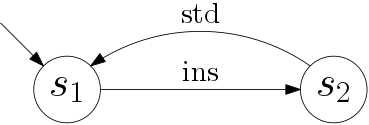
\includegraphics[scale=0.3]{Examples/CoffeeMachine/BasicEuroLTS}
	\caption[Coffee machine LTS]{Coffee machine LTS $C$}
	\label{fig:coffeemachinebasiceurolts}
\end{figure}


\begin{definition}
	\label{def_mu_syntax}
	A modal $\mu$-calculus formula over the set of actions $Act$ and a set of variables $\mathcal{X}$ is defined by
	\[ \varphi = \top\ |\ \bot\ |\ X\ |\ \varphi \vee \varphi\ |\ \varphi \wedge \varphi\ |\ \langle a \rangle \varphi\ |\ [a]\varphi\ |\ \mu X.\varphi\ |\ \nu X.\varphi \]
	with $a \in Act$ and $X \in \mathcal{X}$. 
	
	
	No negations in the language because negations can be pushed inside to the propositions, ie. the $\top$ and $\bot$ elements.
\end{definition}
The modal $\mu$-calculus contains boolean constants $\top$ and $\bot$, propositional operators $\vee$ and $\wedge$, modal operators $\langle \, \rangle$ and $[ \, ]$ and fixpoint operators $\mu$ and $\nu$. A formula is closed when variables only occur in the scope of a fixpoint operator for that variable.

A modal $\mu$-calculus formula can be interpreted with an LTS, this results in a set of states for which the formula holds.
\begin{definition}
	\label{def_mu_sem} For LTS $(S, Act, trans, s_0)$ we inductively define the interpretation of a modal $\mu$-calculus formula $\varphi$, notation
	$[\![ \varphi ]\!]^\eta$, where $\eta : \mathcal{X} \rightarrow \mathcal{P}(S)$ is a logical variable valuation, as a set of states
	where $\varphi$ is valid, by:
	\begin{align*}
	&[\![ \mathit{\top} ]\!]^\eta &&= S\\
	&[\![ \mathit{\bot} ]\!]^\eta &&= \emptyset\\
	&[\![ \varphi_1 \wedge \varphi_2 ]\!]^\eta &&= [\![ \varphi_1 ]\!]^\eta \cap [\![ \varphi_2 ]\!]^\eta \\
	&[\![ \varphi_1 \vee \varphi_2 ]\!]^\eta &&= [\![ \varphi_1 ]\!]^\eta \cup [\![ \varphi_2 ]\!]^\eta\\
	&[\![ \langle a \rangle \varphi ]\!]^\eta &&= \{s \in S|\exists_{s' \in S} s \xrightarrow {a} s' \wedge s' \in [\![ \varphi ]\!]^\eta\}\\
	&[\![ [ a ] \varphi ]\!]^\eta &&= \{s \in S|\forall_{s' \in S} s \xrightarrow {a} s' \implies s' \in [\![ \varphi ]\!]^\eta\}\\
	&[\![ \mu X. \varphi ]\!]^\eta &&= \bigcap_{f \subseteq S}\{f | f = [\![ \varphi ]\!]^{\eta[X:=f]}\}\\
	&[\![ \nu X. \varphi ]\!]^\eta &&= \bigcup_{f \subseteq S}\{f | f = [\![ \varphi ]\!]^{\eta[X:=f]}\}\\
	&[\![ X ]\!]^\eta &&= \eta(X)
	\end{align*}
\end{definition}

Given closed formula $\varphi$, LTS $M = (S, Act, trans, s_0)$ and $s \in S$ we write $(M,s) \models \varphi$ iff $s \in [\![ \varphi ]\!]^\eta$ for $M$, we say that formula $\varphi$ holds for $M$ in state $s$. If formula $\varphi$ holds for $M$ in the initial state we say that formula $\varphi$ holds for $M$ and write $M \models \varphi$.

Again consider the coffee machine example (figure \ref{fig:coffeemachinebasiceurolts}) and formula $\varphi = \nu X. \mu Y. ([ins]Y \wedge [std] X)$ (taken from \cite{FamBasedModelCheckingWithMCRL2}) which states that action \textit{std} must occur infinitely often over all runs. Obviously this holds for the coffee machine, therefore we have $C \models \varphi$.

\subsection{Featured transition systems}
A \textit{featured transition system} (FTS) extends the LTS definition to express variability. It does so by introducing \textit{features} and \textit{products} into the definition. Features are options that can be enabled or disabled for the system. A product is a feature assignments, ie. a set of features that is enabled for that product. Not all products are valid, some features might be mutually exclusive and some features might always be required. To express the relation between features one can use feature diagrams as explained in \cite{Classen2013FeaturedTS}. Feature diagrams offer a nice way of expressing which feature assignments are valid, however for simplicity we will represent the collection of valid products simply with a set of feature assignments. Finally FTSs guard every transition with a boolean expression over the set of features. We have the following definition, based on \cite{Classen2013FeaturedTS}:
\begin{definition}
	\label{def_fts}A featured transition system (FTS) is a tuple $M = (S, Act, trans, s_0, N, P, \gamma)$, where:
	\begin{itemize}
		\item $S, Act, trans, s_0$ are defined as in an LTS,
		\item $N$ is a non-empty set of features,
		\item $P \subseteq \mathcal{P}(N)$ is a set of products, ie. feature assignments, that are valid,
		\item $\gamma : trans \rightarrow \mathbb{B}(N)$ is a total function, labelling each transition with a boolean expression over the features. A product $p \in \mathcal{P}(N)$ satisfying the boolean expression of transition $t$ is denoted by $p \models \gamma(t)$. The boolean expression that is satisfied by any feature assignment is denoted by $\top$, ie $p \models \top$ for any $p$.
		
		A transition $s \xrightarrow a s'$ and $\gamma((s,a,s')) = f$ is denoted by $s \xrightarrow {a | f} s'$. 
	\end{itemize}
\end{definition}
\begin{figure}[h]
\centering
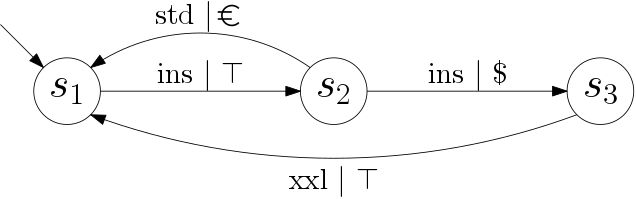
\includegraphics[scale=0.3]{Examples/CoffeeMachine/FTS}
\caption[Coffee machine LTS]{Coffee machine FTS $C$}
\label{fig:coffeemachinefts}
\end{figure}

Consider the example in figure \ref{fig:coffeemachinefts} (directly taken from \cite{FamBasedModelCheckingWithMCRL2}) which shows an FTS for a coffee machine For this example we have two features $N = \{\$, \officialeuro\}$ and two valid products $P = \{\{\$\},\{\officialeuro\}\}$.

An FTS expresses the behaviour of multiple products, we can derive the behaviour of a single product by simply removing all the transitions from the FTS for which the product doesn't satisfy the feature expression guarding the transition. We call this a \textit{projection} \cite{Classen2013FeaturedTS}.

\begin{definition}
	\label{def_fts_proj}
	The projection of an FTS $M = (S, Act, trans, s_0, N, P, \gamma)$ to a product $p \in P$, noted $M_{|p}$, is the LTS $M'=(S,Act,trans', s_0)$, where $trans' = \{t \in trans\ |\ p \models \gamma(t)\}$.
\end{definition}
The coffee machine example can be projected to its two products, which results in the LTSs in figure \ref{fig:cofeemachineftsproj}.
\begin{figure}[h]
	\centering
	\begin{subfigure}{.5\textwidth}
		\centering
		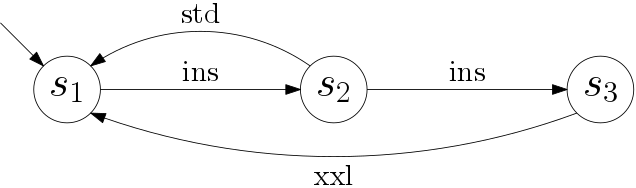
\includegraphics[width=1\linewidth]{Examples/CoffeeMachine/FTSProjDollar}
		\caption[$C_{|\{\$\}}$]{$C$ projected to the dollar product: $C_{|\{\$\}}$}
		\label{fig:coffeemachineftsprojdollar}
	\end{subfigure}%
	\begin{subfigure}{.5\textwidth}
		\centering
		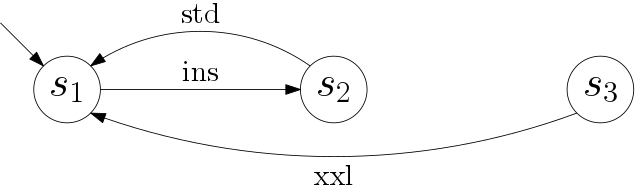
\includegraphics[width=1\linewidth]{Examples/CoffeeMachine/FTSProjEuro}
		\caption[$C_{|\{\$\}}$]{$C$ projected to the euro product: $C_{|\{\officialeuro\}}$}
		\label{fig:coffeemachineftsprojeuro}
	\end{subfigure}
	\caption{Projections of the coffee machine FTS}
	\label{fig:cofeemachineftsproj}
\end{figure}
\subsection{FTS verification question}
When verifiying an FTS against a model $\mu$-calculus formula $\varphi$, we are trying to answer the question: For which products in the FTS does its projection satisfy $\varphi$? Formally, given FTS $M = (S, Act, trans, s_0, N, P, \gamma)$ and modal $\mu$-calculus formula $\varphi$ we want to find $P_s \subseteq P$ such that:
\begin{itemize}
	\item for every $p \in P_s$ we have $M_{|p} \models \varphi$ and
	\item for every $p \in P \backslash P_s$ we have $M_{|p} \not\models \varphi$.
\end{itemize}
Furthermore a counterexample for every $p \in P \backslash P_s$ is preferred.

\section{Verification using parity games}
Verifying LTSs against a modal $\mu$-calculus formula can be done by solving a \textit{parity game}. This is done by translating an LTS in combination with a formula to a parity game, the solution of the parity game provides the information needed to conclude if the model satisfies the formula. This relation is depicted in figure \ref{fig:ltsverificationusingpg}. This technique is well known and well studied, in this section we will first look at parity games, the translation from LTS and formula to a parity game and finally what we can do with this technique to verify FTS.
\begin{figure}[h]
	\centering
	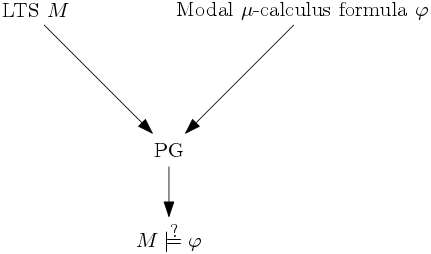
\includegraphics[scale=0.5]{Diagrams/LTSVerificationUsingPG}
	\caption[LTS verification using PG]{LTS verification using PG}
	\label{fig:ltsverificationusingpg}
\end{figure}


\subsubsection{Parity games}
\begin{definition}
	\label{def_PG}\cite{Bradfield2018}
	A parity game (PG) is a tuple $(V, V_0, V_1, E, \Omega)$, where:
	\begin{itemize}
		\item $V = V_0 \cup V_1$ and $V_0 \cap V_1 = \emptyset$,
		\item $V_0$ is the set of vertices owned by player $0$,
		\item $V_1$ is the set of vertices owned by player $1$, 
		\item $E \subseteq V \times V$ is the edge relation,
		\item $\Omega :  V \rightarrow \mathbb{N}$ is a priority assignment.
	\end{itemize}
\end{definition}
A parity game is played by players 0 and 1. We write $\alpha \in \{0,1\}$ to denote an arbitrary player. We write $\overline{\alpha}$ to denote $\alpha$'s opponent, ie. $\overline{0} = 1$ and $\overline{1} = 0$.

 A play starts with placing a token on vertex $v \in V$. Player $\alpha$ moves the token if the token is on a vertex owned by $\alpha$, ie. $v \in V_\alpha$. The token can be moved to $w \in V$, with $(v,w) \in E$. A series of moves results in a sequence of vertices, called a path. For path $\pi$ we write $\pi_i$ to denote the $i^{\text{th}}$ vertex in path $\pi$. A play ends when the token is on vertex $v \in V_\alpha$ and $\alpha$ can't move the token anywhere, in this case player $\overline{\alpha}$ wins the play. If the play results in an infinite path $\pi$ then we determine the highest priority that occurs infinitely often in this path, formally
\[ \max\{ p \ |\ \forall_j \exists_i j < i \wedge p = \Omega(\pi_i) \}\] 
If the highest priority is odd then player $1$ wins, if it is even player $0$ wins.
\begin{figure}[h]
	\centering
	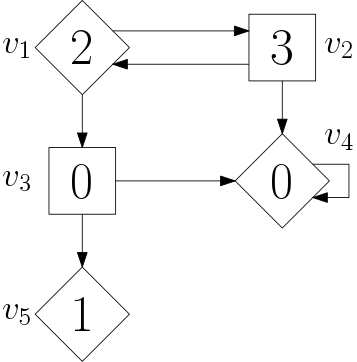
\includegraphics[scale=0.3]{Examples/SimplePG/PG}
	\caption[Parity game example]{Parity game example}
	\label{fig:simplepgpg}
\end{figure}

Figure \ref{fig:simplepgpg} shows an example of a parity game. We usually depict the vertices owned by player $0$ by diamonds and vertices owned by player $1$ by boxes, the priority is depicted inside the vertices. If the game starts by placing a token on $v_1$ we can consider the following exemplary paths:
\begin{itemize}
	\item $\pi = v_1v_3v_5$ is won by player $1$ since player $0$ can't move at $v_5$.
	\item $\pi = (v_1v_2)^\omega$ is won by player $1$ since the highest priority occurring infinitely often is 3.
	\item $\pi = v_1v_3(v_4)^\omega$ is won by player $0$ since the highest priority occurring infinitely often is $0$.
\end{itemize}


A strategy for player $\alpha$ is a function $\sigma : V^*V_\alpha \rightarrow V$ that maps a path ending in a vertex owned by player $\alpha$ to the next vertex. Parity games are positionally determined \cite{Bradfield2018}, therefore a strategy $\sigma: V_\alpha \rightarrow V$ that maps the current vertex to the next vertex is sufficient. 

A strategy $\sigma$ for player $\alpha$ is winning from vertex $v$ iff any play that results from following $\sigma$ results in a win for player $\alpha$. The graph can be divided in two partitions $W_0 \subseteq V$ and $W_1 \subseteq V$, called winning sets. Iff $v \in W_\alpha$ then player $\alpha$ has a winnings strategy from $v$. Every vertex in the graph is either in $W_0$ or $W_1$ \cite{Bradfield2018}. Furthermore finite parity games are decidable \cite{Bradfield2018}.


\subsubsection{Creating parity games}
A parity game can be created from a combination of an LTS and a modal $\mu$-calculus formula. To do this we introduce some auxiliary definitions regarding the modal $\mu$-calculus.

First we introduce the notion of unfolding, a fixpoint formula $\mu X . \varphi$ can be unfolded resulting in formula $\varphi$ where every occurrence of $X$ is replaced by $\mu X . \varphi$, denoted by $\varphi [ X:= \mu X . \varphi]$. A fixpoint formula is equivalent to its unfolding \cite{Bradfield2018}, ie. for some LTS $[\![\mu X . \varphi]\!]^\eta = [\![\varphi[X:=\mu X . \varphi]]\!]^\eta$. The same holds for the fixpoint operator $\nu$.

Next we define the Fischer-Ladner closure for a closed $\mu$-calculus formula 
\cite{STREETT1989249,FISCHER1979194}. The Fischer-Ladner closure of $\varphi$ is the set $\textit{FL}(\varphi)$ of closed formula's containing at least $\varphi$. Furthermore for every formula $\psi$ in $\textit{FL}(\varphi)$ it holds that for every direct subformula $\psi'$ of $\psi$ there is a formula in $\textit{FL}(\varphi)$ that is equivalent to $\psi'$.
\begin{definition}
	\label{def_FLClosure}
	The Fischer-Ladner closure of closed $\mu$-calculus formula $\varphi$ is the smallest set $\textit{FL}(\varphi)$ satisfying the following constraints:
	\begin{itemize}
		\item $\varphi \in \textit{FL}(\varphi)$,
		\item if $\varphi_1 \vee \varphi_2 \in \textit{FL}(\varphi)$ then $\varphi_1 ,\varphi_2 \in \textit{FL}(\varphi)$,
		\item if $\varphi_1 \wedge \varphi_2 \in \textit{FL}(\varphi)$ then $\varphi_1 ,\varphi_2 \in \textit{FL}(\varphi)$,
		\item if $\langle a \rangle \varphi' \in \textit{FL}(\varphi)$ then $\varphi' \in \textit{FL}(\varphi)$,
		\item if $[ a ] \varphi' \in \textit{FL}(\varphi)$ then $\varphi' \in \textit{FL}(\varphi)$,
		\item if $\mu X . \varphi' \in \textit{FL}(\varphi)$ then $\varphi'[X:= \mu X . \varphi'] \in \textit{FL}(\varphi)$ and
		\item if $\nu X . \varphi' \in \textit{FL}(\varphi)$ then $\varphi'[X:= \nu X . \varphi'] \in \textit{FL}(\varphi)$.
		
	\end{itemize}
\end{definition}

Finally we define alternating depth.
\begin{definition}\cite{Bradfield2018}
	The dependency order on bound variables of $\varphi$	is the smallest partial order such that $X \leq_\varphi Y$ if $X$ occurs free in $\sigma Y. \psi$ . The alternation depth of a $\mu$-variable X in formula $\varphi $ is the maximal length of a chain $X_1 \leq_\varphi  \dots \leq_\varphi X_n$ where $X = X_1$, variables $X_1, X_3, \dots$ are $\mu$-variables and variables $X_2, X_4, \dots$ are $\nu$-variables. The alternation depth of a $\nu$-variable is defined similarly. The alternation depth of formula $\varphi$, denoted $adepth(\varphi)$, is the maximum of the alternation depths of the variables bound in $\varphi$, or zero if there are no fixpoints.
\end{definition}
Consider the example formula $\varphi = \nu X. \mu Y. ([ins]Y \wedge [std] X)$ which states that for an LTS with $Act = \{ ins, std\}$ the action \textit{std} must occur infinitely often over all runs. Since $X$ occurs free in $\mu Y. ([ins] Y \wedge [std]X)$ we have $adepth(Y) = 1$ and $adepth(X) = 2$. As shown in \cite{Bradfield2018} it holds that formula $\mu X. \psi$ has the same alternation depth as its unfolding $\psi[X:=\mu X. \psi]$. Similarly for the greatest fixpoint.



We can now define the transformation from an LTS and a formula to a parity game.
\begin{definition}
	\label{def_LTS2PG}\cite{Bradfield2018}
	LTS2PG($M, \varphi$) converts LTS $M = (S, Act, trans, s_0)$ and closed formula $\varphi$ to a PG $(V, V_0, V_1, E, \Omega)$.
	
	A vertex in the parity game is represented by a pair $(s, \psi)$ where $s \in S$ and $\psi$ is a modal $\mu$-calculus formula. We will create a vertex for every state with every formula in the Fischer-Ladner closure of $\varphi$. We define the set of vertices:
	\[ V = S \times \textit{FL}(\varphi) \]
	
	We create the parity game with the smallest set $E$ such that:
	\begin{itemize}
		\item $V = V_0 \cup V_1$,
		\item $V_0 \cap V_1 = \emptyset$ and
		\item for every $v = (s, \psi) \in V$ we have:
		\begin{itemize}
			\item If $\psi = \top$ then $v \in V_1$.
			\item If $\psi = \bot$ then $v \in V_0$.
			\item If $\psi = \psi_1 \vee \psi_2$ then:
			\subitem $v \in V_0$,
			\subitem $(v, (s,\psi_1)) \in E$ and
			\subitem $(v, (s,\psi_2)) \in E$.
			\item If $\psi = \psi_1 \wedge \psi_2$ then:
			\subitem $v \in V_1$,
			\subitem $(v, (s,\psi_1)) \in E$ and
			\subitem $(v, (s,\psi_2)) \in E$.
			\item If $\psi = \langle a \rangle \psi'$ then $v \in V_0$ and for every $s \xrightarrow{ a} s'$ we have $(v, (s', \psi')) \in E$.
			\item If $\psi = [ a ] \psi'$ then $v \in V_1$ and for every $s \xrightarrow{ a} s'$ we have  $(v, (s', \psi')) \in E$.
			\item If $\psi = \mu X. \psi'$ then $(v, (s, \psi'[X:=\mu X. \psi'])) \in E$.
			\item If $\psi = \nu X. \psi'$ then $(v, (s, \psi'[X:=\nu X. \psi'])) \in E$.
		\end{itemize}
	\end{itemize}
	Since the Fischer-Ladner formula's are closed we never get the case $\psi = X$.
	
	Finally we have $\Omega(s, \psi) = \begin{cases}
	2 \lfloor adepth(X) / 2 \rfloor & \text{if } \psi = \nu X. \psi'\\
	2 \lfloor adepth(X) / 2 \rfloor + 1 & \text{if } \psi = \mu X. \psi'\\
	0 & \text{otherwise}
	\end{cases}$
\end{definition}
\begin{figure}[h]
	\centering
	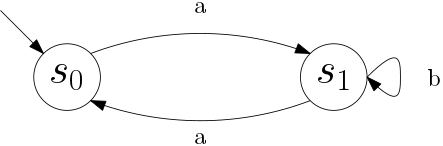
\includegraphics[scale=0.3]{Examples/ExamleVerification/LTSprojempty}
	\caption[LTS $M$]{LTS $M$}
	\label{fig:exverltsprojempty}
\end{figure}\begin{figure}[h]
\centering
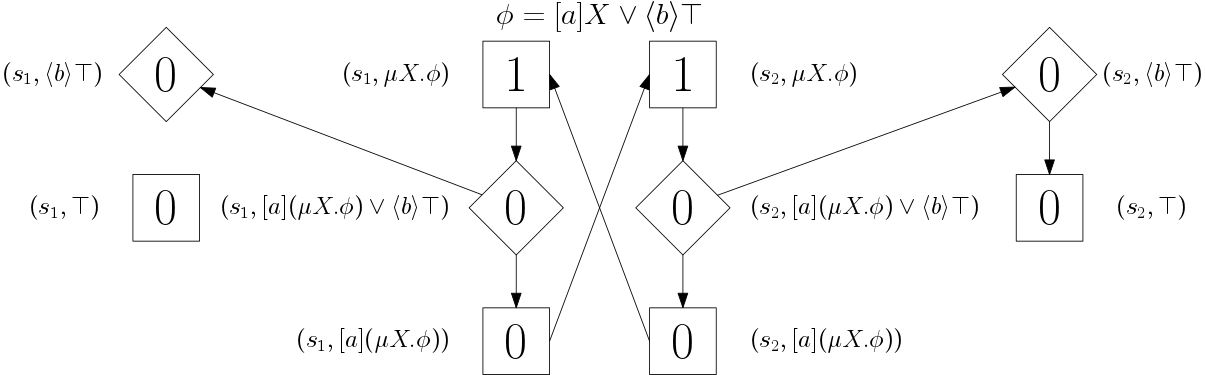
\includegraphics[scale=0.3]{Examples/ExamleVerification/PG}
\caption[Parity game $LTS2PG(M, \varphi)$]{Parity game $LTS2PG(M, \varphi)$}
\label{fig:exverpg}
\end{figure}
Consider LTS $M$ in figure \ref{fig:exverltsprojempty} and formula $\varphi = \mu X.([a]X \vee \langle b \rangle \top)$ expressing that on any path reached by $a$'s we can eventually do a $b$ action. We will use this as a working example in the next few sections. The resulting parity game is depicted in figure \ref{fig:exverpg}. Solving this parity game results in the following winning sets:%
\begin{align*}
	W_0 = \{& (s_1, \mu X.\phi),\\
	& (s_1, [a](\mu X. \phi) \vee \langle b \rangle \top),\\
	& (s_1, [a](\mu X. \phi)),\\
	& (s_1, \top),\\
	& (s_2, \mu X.\phi),\\
	& (s_2, [a](\mu X. \phi) \vee \langle b \rangle \top),\\
	& (s_2, [a](\mu X. \phi)),\\
	& (s_2, \langle b \rangle \top),\\
	& (s_2, \top)
	\}\\
	W_1 = \{& (s_1, \langle b \rangle \top )\}
\end{align*}
With the strategies $\sigma_0$ for player $0$ and $\sigma_1$ for player $1$ being (vertices with one outgoing edge are omitted):
\begin{align*}
\sigma_0 = \{
&(s_1, [a](\mu X. \phi) \vee \langle b \rangle \top) \mapsto (s_1, [a] (\mu X. \phi)), \\
&(s_2, [a](\mu X. \phi) \vee \langle b \rangle \top) \mapsto (s_2, \langle b \rangle \top) \} \\
\sigma_1 = \{&\} \\
\end{align*}

State $s$ in LTS $M$ only satisfies $\varphi$ iff player $0$ has a winning strategy from vertex $(s, \varphi)$. This is formally stated in the following theorem which is proven in \cite{Bradfield2018}.
\begin{theorem}
	\label{the_LTS_PG_REL}Given LTS $M = (S, Act, trans, s_0)$, modal $\mu$-calculus formula $\varphi$ and state $s \in S$ it holds that $(M, s) \models \varphi$ iff $s \in W_0$ for the game $LTS2PG(M, \varphi)$.
\end{theorem}

\subsubsection{FTSs and parity games}
Using the theory we have seen thus far we can verify FTSs by verifying every projection of the FTS to a valid product. This relation is depicted in the following diagram where $\Pi$ indicates a projection:
\\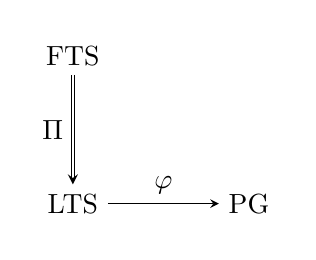
\begin{tikzpicture}
\matrix (m) [matrix of math nodes,row sep=4em,column sep=4em,minimum width=2em]
{
	\text{FTS} \\
	\text{LTS} & \text{PG} \\};
\path[-stealth]
(m-1-1) edge [double] node [left] {$\Pi$} (m-2-1)
(m-2-1.east|-m-2-2) edge node [above] {$\varphi$}
(m-2-2)
;
\end{tikzpicture}\\
As mentioned before verifying products dependently is potentially more efficient. In the next two sections we define an extension to parity games, namely \textit{variability parity games} (VPGs) which can be used to verify an FTS. We will translate an FTS and a formula into a VPG which solution will provide the information needed to conclude for which products the FTS satisfies the formula.


\section{Featured parity games}
Before we can define variability parity games we first define \textit{featured parity games} (FPG), featured parity games extend the definition of parity games to capture the variability represented in an FTS. It uses the same concepts as FTSs: features, products and a function that guards edges. In this section we will introduce the definition of FPGs and show that solving them answers the verification questions for FTS: For which products in the FTS does its projection satisfy $\varphi$?

First we introduce the definition of an FPG:
\begin{definition}
	\label{def_FPG}
	A featured parity game (FPG) is a tuple $(V,V_0, V_1, E, \rho, N, P, \gamma)$, where:
	\begin{itemize}
		\item $V = V_0 \cup V_1$ and $V_0 \cap V_1 = \emptyset$,
		\item $V_0$ is the set of vertices owned by player $0$,
		\item $V_1$ is the set of vertices owned by player $1$, 
		\item $E \subseteq V \times V$ is the edge relation,
		\item $\rho :  V \rightarrow \mathbb{N}$ is a priority assignment,
		\item $N$ is a set of features,
		\item $P \subseteq \mathcal{P}(N)$ is a set of products, ie. feature assignments, for which the game can be played,
		\item $\gamma : E \rightarrow \mathbb{B}(N)$ is a total function, labelling each edge with a Boolean expression over the features.
	\end{itemize}
\end{definition}
An FPG is played similarly to a PG, however the game is played for a specific product $p \in P$. Player $\alpha$ can only move the token from $v \in V_\alpha$ to $w \in V$ if $(v,w) \in E$ and $p \models \gamma(v,w)$.

A game played for product $p \in P$ results in winnings sets $W_0^p$ and $W_1^p$, which are defined similar to the $W_0$ and $W_1$ winning sets for parity games.

An FPG can simply be projected to a product $p$ by removing the edges that are not satisfied by $p$.
\begin{definition}
	\label{def_FPG_proj}
The projection from FPG $G = (V,V_0, V_1, E, \rho, N, P, \gamma)$ to a product $p \in P$, noted $G_{|p}$, is the parity game $(V,V_0,V_1, E', \rho)$ where $E' = \{ e \in E\ |\ p \models \gamma(e) \}$.
\end{definition}

Playing FPG $G$ for a specific product $p\in P$ is the same as playing the PG $G_{|p}$. Any path that is valid in $G$ for $p$ is also valid in $G_{|p}$ and vice versa. Therefore the strategies are also interchangeable, furthermore the winning sets $W_\alpha$ for $G_{|p}$ and $W_\alpha^p$ for $G$ are identical. Since parity games are positionally determined so are FPGs. Similarly, since finite parity games are decidable, so are finite FPGs.

Solving an FPG means determining winning sets for every valid product in the FPG.
\subsection{Creating featured parity games}
An FPG can be created from an FTS in combination with a model $\mu$-calculus formula. We translate an FTS to an FPG by first creating a PG from the transition system as if there were no transition guards, next we apply the same guards to the FPG as are present in the FTS for edges that originate from transitions. The features and valid products in the FPG are identical to those in the FTS.
\begin{definition}
	\label{def_FTS2FPG}
	$FTS2FPG(M, \varphi)$ converts FTS $M = (S, Act, trans, s_0, N, P, \gamma)$ and closed formula $\varphi$ to FPG $(V, V_0, V_1, E, \rho, N, P, \gamma')$.
	
	We have $(V, V_0, V_1, E, \rho)$ = LTS2PG($(S, Act, trans, s_0), \varphi$) and
	\[ \gamma'((s, \psi),(s', \psi')) = \begin{cases}
	\gamma(s,a,s') & \text{if }\psi = \langle a \rangle \psi'\text{ or }\psi = [a]\psi' \\
	\top & \text{otherwise}
	\end{cases}\]
\end{definition}
Consider our working example which we extend to an FTS depicted in figure \ref{fig:exverfts}, for this example we have features $N = \{f, g\}$ and products $P = \{\emptyset, \{f\},\{f,g\}\}$.
\begin{figure}[h]
	\centering
	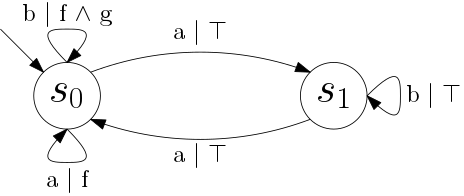
\includegraphics[scale=0.3]{Examples/ExamleVerification/FTS}
	\caption[FTS $M$]{FTS $M$}
	\label{fig:exverfts}
\end{figure}
\begin{figure}[h]
	\centering
	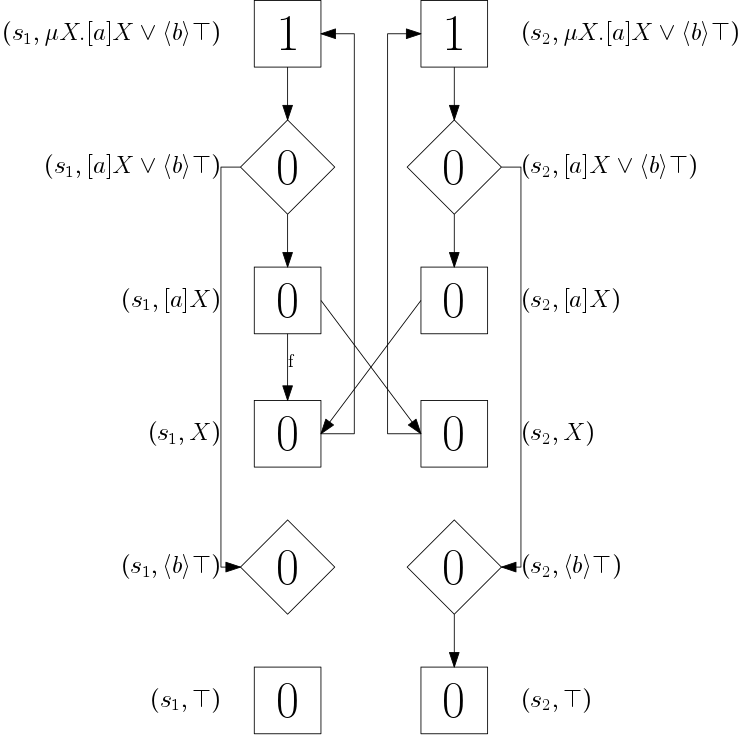
\includegraphics[scale=0.3]{Examples/ExamleVerification/FPG}
	\caption[FPG for $M$ and $\varphi$]{FPG for $M$ and $\varphi$}
	\label{fig:exverfpg}
\end{figure}
We can translate this FTS with formula $\varphi = \mu X. ([a] X \vee \langle b \rangle \top)$ to an FPG depicted in figure \ref{fig:exverfpg}. As we can see from the FTS if feature $f$ is enabled and $g$ is disabled then we have an infinite path of $a$'s where $b$ is never enabled, therefore $\varphi$ doesn't hold for $M_{|\{f\}}$. If $g$ is enabled however we can always do a $b$ so $\varphi$ holds for $M_{|\{f,g\}}$. As we have seen $\varphi$ does hold for $M_{|\emptyset}$. For the product $\emptyset$ we have the same winning set as before:
\begin{align*}
W_0^\emptyset = \{& (s_1, \mu X.[a]X \vee \langle b \rangle \top),\\
& (s_1, [a]X \vee \langle b \rangle \top),\\
& (s_1, [a]X),\\
& (s_1, X),\\
& (s_1, \top),\\
& (s_2, \mu X.[a]X \vee \langle b \rangle \top),\\
& (s_2, [a]X \vee \langle b \rangle \top),\\
& (s_2, [a]X),\\
& (s_2, X),\\
& (s_2, \langle b \rangle \top),\\
& (s_2, \top)
\}\\
W_1^\emptyset = \{& (s_1, \langle b \rangle \top )\}
\end{align*}
In the FPG we can see that if $f$ is enabled and $g$ is disabled then player $1$ can move the token from $(s_1, [a]X)$ to $(s_1,X)$. This results in player $0$ either moving the token to $(s_1, \langle b \rangle \top)$ and losing or an infinite path where $1$ occurs infinitely often which is also player $1$ wins. For product $\{f\}$ we have winning sets:
\begin{align*}
W_0^{\{f\}} = \{
& (s_1, \top),\\
& (s_2, \mu X.[a]X \vee \langle b \rangle \top),\\
& (s_2, [a]X \vee \langle b \rangle \top),\\
& (s_2, X),\\
& (s_2, \langle b \rangle \top),\\
& (s_2, \top)
\}\\
W_1^{\{f\}} = \{& (s_1, \mu X.[a]X \vee \langle b \rangle \top),\\
& (s_1, [a]X \vee \langle b \rangle \top),\\
& (s_1, [a]X),\\
& (s_1, X),\\
& (s_1, \langle b \rangle \top ),\\
& (s_2, [a]X)\}
\end{align*}
However if $g$ is also enabled then player $0$ wins in $(s_1, \langle b \rangle \top)$, thus giving the following winning sets:
\begin{align*}
W_0^{\{f,g\}} = \{& (s_1, \mu X.[a]X \vee \langle b \rangle \top),\\
& (s_1, [a]X \vee \langle b \rangle \top),\\
& (s_1, [a]X),\\
& (s_1, X),\\
& (s_1, \langle b \rangle \top ),\\
& (s_1, \top),\\
& (s_2, \mu X.[a]X \vee \langle b \rangle \top),\\
& (s_2, [a]X \vee \langle b \rangle \top),\\
& (s_2, [a]X),\\
& (s_2, X),\\
& (s_2, \langle b \rangle \top),\\
& (s_2, \top)
\}\\
W_1^{\{f,g\}} = \{\}
\end{align*}

In the next section we will show how the winning sets relate to the model verification question.


\subsection{FTS verification using FPG}
We can create an FPG from an FTS and project it to a PG, this is shown in the following diagram:\\
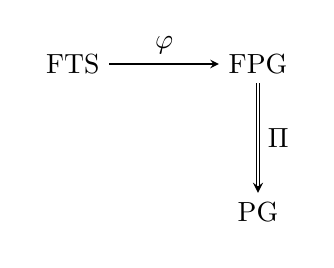
\begin{tikzpicture}
\matrix (m) [matrix of math nodes,row sep=4em,column sep=4em,minimum width=2em]
{
	\text{FTS} & \text{FPG} \\
	\  & \text{PG} \\};
\path[-stealth]
(m-1-1)
edge node [above] {$\varphi$} (m-1-2)

(m-1-2) edge [double] node [right] {$\Pi$} (m-2-2)
;
\end{tikzpicture}\\
Earlier we saw that we could also derive a PG by projecting the FTS to a product and then translation the resulting LTS to a PG, depicted by the following diagram:
\\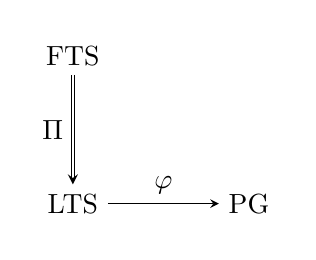
\begin{tikzpicture}
\matrix (m) [matrix of math nodes,row sep=4em,column sep=4em,minimum width=2em]
{
	\text{FTS} \\
	\text{LTS} & \text{PG} \\};
\path[-stealth]
(m-1-1) edge [double] node [left] {$\Pi$} (m-2-1)
(m-2-1.east|-m-2-2) edge node [above] {$\varphi$}
(m-2-2)
;
\end{tikzpicture}\\
We will now show that the resulting parity games are identical.
\begin{theorem}
	\label{the_PGsubPGA} Given:
	\begin{itemize}
		\item FTS $M = (S,Act, trans, s_0, N, P, \gamma)$,
		\item a closed modal mu-calculus formula $\varphi$,
		\item a product $p \in P$
	\end{itemize}
	it holds that the parity games LTS2PG($M_{|p}, \varphi$) and FTS2FPG($M, \varphi$)$_{|p}$  are identical.
	\begin{proof}
		Let $G^F = FTS2FPG(M, \varphi) = (V^F, V_0^F, V_1^F, E^F, \rho^F, N, P, \gamma')$, using definition \ref{def_FTS2FPG}, and $G^F_{|p} = (V^F, V_0^F, V_1^F, {E^F}', \rho^F)$, using definition \ref{def_FPG_proj}. Furthermore we have $M_{|p} = (S, Act, trans', s_0)$ and we let $G =  LTS2PG(M_{|p}, \varphi) = (V, V_0, V_1, E, \rho)$. We depict the different transition systems and games in the following diagram.
		
		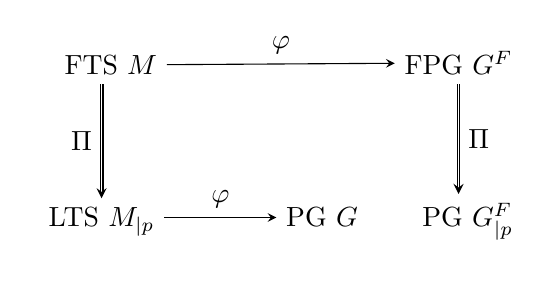
\begin{tikzpicture}
		\matrix (m) [matrix of math nodes,row sep=4em,column sep=1em,minimum width=2em]
		{
			\text{\ \ FTS }M & \  &\ & \text{FPG } G^F  \\
			\text{LTS }M_{|p} & \ & \text{PG } G & \text{\ \ PG }G_{|p}^F \\};
		\path[-stealth]
		(m-1-1) edge [double] node [left] {$\Pi$} (m-2-1)
		edge node [above] {$\varphi$} (m-1-4)
		(m-2-1.east|-m-2-3) edge node [above] {$\varphi$}
		(m-2-3)
		(m-1-4) edge [double] node [right] {$\Pi$} (m-2-4);
		\end{tikzpicture}\\
		We will prove that $G = G_{|p}^F$. We first note that game $G$ is created by 
		\[  (V, V_0, V_1, E, \rho) = LTS2PG((S, Act, trans', s_0),\varphi) \]
		and the vertices, edges and priorities of game $G^F$ are created by 
		\[ (V^F, V_0^F, V_1^F, E^F, \rho^F) = LTS2PG((S,Act, trans, s_0), \varphi)\]
		Using the definition of LTS2PG (\ref{def_LTS2PG}) we find that the vertices and the priorities only depend on the states in $S$ and the formula $\varphi$, since these are identical in the above two statements we immediately get $V = V^F, V_0 = V_0^F, V_1 = V_1^F$ and $\rho = \rho^F$. The vertices and priorities don't change when an FTS is projected, therefore $G_{|p}^F$ has the same vertices and priorities as $G^F$.
		
		Now we are left with showing that $E = {E^F}'$ in order to conclude that that $G = G^F_{|p}$. We will do this by showing $E \subseteq {E^F}'$ and $E \supseteq {E^F}'$.
		
		First let $e \in E$. Note that a vertex in the parity game is represented by a pair of a state and a formula. So we can write $e = ((s,\psi),(s',\psi'))$. To show that $e \in {E^F}'$ we distinguish two cases:
		\begin{itemize}
			\item  If $\psi = \langle a \rangle \psi_1$ or $\psi = [a] \psi_1$ then there exists an $a \in Act$ such that $(s,a,s') \in trans'$. Using definition the FTS projection definition (\ref{def_fts_proj}) we get $(s,a,s') \in trans$ and $p \models \gamma(s,a,s')$. Using the $FTS2FPG$ definition (\ref{def_FTS2FPG}) we find that $\gamma'((s,\psi),(s',\psi')) = \gamma(s,a,s')$ and therefore $p \models \gamma'((s,\psi),(s',\psi'))$. Now using the FPG projection definition (\ref{def_FPG_proj}) we find $((s,\psi),(s',\psi')) \in {E^F}'$.
			\item Otherwise the existence of the edge does not depend on the $trans$ parameter and therefore $((s,\psi),(s',\psi')) \in {E^F}'$ if $(s,\psi) \in V^F$, since $V^F = V$ we have $(s,\psi) \in V^F$.
		\end{itemize}
		We can conclude that $E \subseteq {E^F}'$, next we will show $E \supseteq {E^F}'$. Let $e = ((s,\psi),(s',\psi')) \in {E^F}'$. We distinguish two cases:
		\begin{itemize}
			\item If $\psi = \langle a \rangle \psi_1$ or $\psi = [a] \psi_1$ then there exists an $a \in Act$ such that $(s,a,s') \in trans$. Using the FPG projection definition (\ref{def_FPG_proj}) we get $p \models \gamma'(s,a,s')$. Using the $FTS2FPG$ definition (\ref{def_FTS2FPG}) we get $p \models \gamma(s,a,s')$. Using the projection definition (\ref{def_FTS2FPG}) we get $(s,a,s') \in trans'$ and therefore $((s,\psi),(s',\psi'))\in E$.
			\item Otherwise the existence of the edge does not depend on the $trans$ parameter and therefore $((s,\psi),(s',\psi')) \in E$ if $(s,\psi) \in V$, since $V^F = V$ we have $(s,\psi) \in V$.
		\end{itemize}
	\end{proof}
\end{theorem}

Having proven this we can visualize the relation between the different games and transition systems in the following diagram:
\\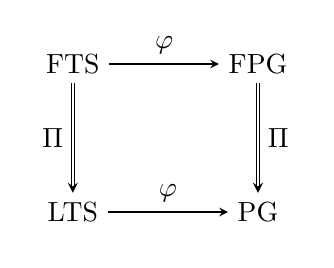
\begin{tikzpicture}
\matrix (m) [matrix of math nodes,row sep=4em,column sep=4em,minimum width=2em]
{
	\text{FTS} & \text{FPG} \\
	\text{LTS} & \text{PG} \\};
\path[-stealth]
(m-1-1) edge [double] node [left] {$\Pi$} (m-2-1)
edge node [above] {$\varphi$} (m-1-2)
(m-2-1.east|-m-2-2) edge node [above] {$\varphi$}
(m-2-2)
(m-1-2) edge [double] node [right] {$\Pi$} (m-2-2)
;
\end{tikzpicture}\\
Finally we prove that solving an FTS, ie. finding winning sets for all products, answers the verification question.
\begin{theorem}
	\label{the_FPG_ver_FTS}
	Given:
	\begin{itemize}
		\item FTS $M = (S, Act, trans, s_0, N, P, \gamma)$,
		\item closed modal mu-calculus formula $\varphi$,
		\item product $p \in P$ and
		\item state $s \in S$
	\end{itemize}
	it holds that $M_{|p}, s \models \varphi$ if and only if $(s, \varphi) \in W_0^p$ in FTS2FPG($M, \varphi$).
	\begin{proof}
		The winning set $W_\alpha^p$ is equal to winning set $W_\alpha$ in $FTS2FPG(M, \varphi)_{|p}$, for any $\alpha \in \{0,1\}$, using the FPG definition (\ref{def_FPG}). Using theorem \ref{the_PGsubPGA} we find that the game $FTS2FPG(M, \varphi)_{|p}$ is equal to the game $LTS2PG(M_{|p}, \varphi)$, obviously their winning sets are also equal. Using the well studied relation between parity games and LTS verification, stated in theorem \ref{the_LTS_PG_REL}, we know that $M_{|p}, s \models \varphi$ if and only if $(s, \varphi) \in W_0$ in game $LTS2PG(M_{|p},\varphi)$. Winning set $W_\alpha^p$ is equal to $W_\alpha$, therefore the theorem holds.
	\end{proof}
\end{theorem}

Revisiting our prior example we can see the theorem in action by noting that $M_{|\emptyset} \models \varphi$ , $M_{|\{f\}} \not\models \varphi$ and $M_{|\{f,g\}} \models \varphi$. This is reflected by the vertex $(s_1, \mu X. [a]X \vee \langle b \rangle \top)$ being present in $W_0^\emptyset$ and $W_0^{\{f,g\}}$ but not in $W_0^{\{f\}}$.

\section{Variability parity games}
Next we will introduce \textit{variability parity games} (VPGs). VPGs are very similar to FPGs, however VPGs use configurations instead of features and products to express variability. This gives a syntactically more pleasant representation that is not solely tailored for FTSs. Furthermore in VPGs deadlocks are removed, by doing so VPG plays can only result in infinite paths and no longer in finite paths.

Later we will show the relation between VPGs and FTS verification, which is similar to the relation between FPGs and FTS verification. First we introduce VPGs.
\begin{definition}
\label{def_VPG}
A variability parity game (VPG) is a tuple $(V,V_0, V_1, E, \Omega, \mathfrak{C}, \theta)$, where:
\begin{itemize}
	\item $V = V_0 \cup V_1$ and $V_0 \cap V_1 = \emptyset$,
	\item $V_0$ is the set of vertices owned by player $0$,
	\item $V_1$ is the set of vertices owned by player $1$, 
	\item $E \subseteq V \times V$ is the edge relation; we assume that $E$ is total, i.e. for all $v\in V$ there is some $w \in V$ such that $(v,w) \in E$,
	\item $\Omega :  V \rightarrow \mathbb{N}$ is a priority assignment,
	\item $\mathfrak{C}$ is a non-empty finite set of configurations,
	\item $\theta : E \rightarrow \mathcal{P}(\mathfrak{C})\ \backslash\ \{0\}$ is the configuration mapping, satisfying for all $v \in V$, $\bigcup\{\theta(v,w)\ |\ (v,w) \in E\} = \mathfrak{C}$.
\end{itemize}
\end{definition}
A VPG is played similarly to a PG, however the game is played for a specific configuration $c \in \mathfrak{C}$. Player $\alpha$ can only move the token from $v \in V_\alpha$ to $w \in V$ if $(v,w) \in E$ and $c \in \theta(v,w)$. Furthermore VPGs don't have deadlocks, therefore every play results in an infinite path.

A game played for configuration $c \in \mathfrak{C}$ results in winning sets $W_0^c$ and $W_1^c$, which are defined similar to the $W_0$ and $W_1$ winning sets for parity games.

Solving a VPG means determining winning sets for every configuration in the VPG.
\begin{definition}
\label{def_VPG_proj} The projection from VPG $G = (V, V_0, V_1, E, \Omega, \mathfrak{C}, \theta)$ to a configuration $c \in \mathfrak{C}$, noted $G_{|c}$, is the parity game $(V, V_0, V_1, E', \Omega)$ where $E' = \{ e\in E\ |\ c \in \theta(e)\}$.
\end{definition}

Playing VPG $G$ for a specific configuration $c \in \mathfrak{C}$ is the same as playing the PG $G_{|c}$. Any path that is valid in $G$ for $c$ is also valid in $G_{|c}$ and vice versa. Therefore the strategies are also interchangeable, furthermore the winning sets $W_\alpha$ for $G_{|c}$ and $W_\alpha^c$ for $G$ are identical. Since parity games are positionally determined so are VPGs. Similarly, since finite parity games are decidable, so are finite VPGs.
\subsection{Creating variability parity games}
We will define a translation from an FPG to a VPG. To do so we use the set of valid products as the set of configurations. Furthermore we make the FPG deadlock free, this is done by creating two losing vertices $l_0$ and $l_1$ such that player $\alpha$ loses when the token is in vertex $l_\alpha$. Any vertex that can't move for a configuration will get an edge that is admissible for that configuration towards one of the losing vertices.
\begin{definition}
	\label{def_FPG2VPG}
	FPG2VPG($G^F$) converts FPG $G^F = (V^F, V_0^F, V_1^F, E^F, \Omega^F, N, P, \gamma)$ to VPG $G = (V, V_0, V_1, E, \Omega, \mathfrak{C}, \theta)$.
	
	We define $\mathfrak{C} = P$. We create vertices $l_0$ and $l_1$ and define $V_0 = V_0^F \cup \{l_0\}$, $V_1 = V_1^F \cup \{l_1\}$ and $V = V_0 \cup V_1$.
	
	We construct $E$ by first making $E = E^F$ and adding edges $(l_0, l_0)$ and $(l_1, l_1)$ to $E$. Simultaneously we construct $\theta$ by first making $\theta(e) = \{p \in \mathfrak{C}\ |\ p \models \gamma(e)\}$ for every $e \in E^F$. Furthermore $\theta(l_0,l_0) = \theta(l_1,l_1) = \mathfrak{C}$.
	
	Next, for every vertex $v \in V_\alpha$ with $\alpha = \{0,1\}$, we have $C = \mathfrak{C} \backslash \bigcup \{\theta(v,w)\ |\ (v,w) \in E\}$. If $C \neq \emptyset$ then we add $(v, l_\alpha)$ to $E$ and make $\theta(v,l_\alpha) = C$.
	Finally we have 
	\[ \Omega(v) = \begin{cases}
	1  & \text{if } v = l_0 \\
	0 & \text{if } v = l_1 \\
	\Omega^F(v) &\text{otherwise}
	\end{cases} \]
\end{definition}
Again considering our previous working example we can translate the FPG shown in figure \ref{fig:exverfpg} to the VPG shown in figure \ref{fig:exvevpg}. Where $c_0$ is product $\emptyset$, $c_1$ is $\{f\}$ and $c_2$ is $\{f,g\}$.
\begin{figure}[h]
	\centering
	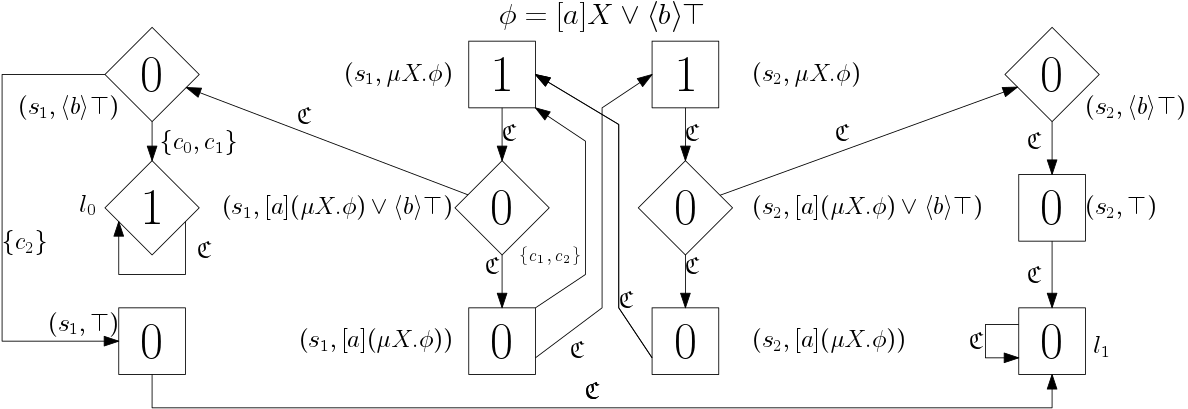
\includegraphics[scale=0.3]{Examples/ExamleVerification/VPG}
	\caption[VPG]{VPG}
	\label{fig:exvevpg}
\end{figure}

\subsection{FTS verification using VPG}
We have shown in theorem \ref{the_FPG_ver_FTS} that we can use an FPG to verify an FTS. Next we will show that a winning set in the FPG $M$ is the subset of the winning set in the VPG $\textit{FPG2VPG}(M)$.
\begin{theorem}
	\label{the_FPG_sub_VPG}
	Given:
	\begin{itemize}
		\item FPG $G^F = (V^F, V_0^F, V_1^F, E^F, \Omega^F, N, P, \gamma)$,
		\item product $p \in P$
	\end{itemize}
	we have for winning sets $Q_\alpha^{p}$ in $G^F$ and $W_\alpha^{p}$ in $\textit{FPG2VPG}(G^F)$ that $Q_\alpha^{p} \subseteq W_\alpha^{p}$ for any $\alpha \in \{0,1\}$.
	\begin{proof}
		Let $G = (V,V_0,V_1, E, \Omega, \mathfrak{C},\theta) = \textit{FPG2VPG}(G^F)$. Consider finite play $\pi$ that is valid in game $G^F$ for product $p$. We have for every $(\pi_i, \pi_{i+1})$ in $\pi$ that $(\pi_i, \pi_{i+1}) \in E^F$ and $p \models \gamma(\pi_i, \pi_{i+1})$. From the $\textit{FPG2VPG}$ definition (\ref{def_FPG2VPG}) it follows that $(\pi_i, \pi_{i+1}) \in E$ and $p \in \theta(\pi_i, \pi_{i+1})$. So we can conclude that path $\pi$ is also valid in game $G$ for configuration $p$. Since the play is finite the winner is determined by the last vertex $v$ in $\pi$, player $\alpha$ wins such that $v \in V_{\overline{\alpha}}$. Furthermore we know, because the play is finite, that there exists no $(v,w) \in E^F$ with $p \models \gamma(v,w)$. From this we can conclude that $(v, l_{\overline{\alpha}}) \in E$ and $p \in \theta(v, l_{\overline{\alpha}})$. Vertex $l_{\overline{\alpha}}$ has one outgoing edge, namely to itself. So finite play $\pi$ will in game $G^F$ results in an infinite play $\pi(l_{\overline{\alpha}})^\omega$. Vertex $l_{\overline{\alpha}}$ has a priority with the same parity as player $\alpha$, so player $\alpha$ wins the infinite play in $G$ for configuration $p$.
		
		Consider infinite play $\pi$ that is valid in game $G^F$ for product $p$. As shown above this play is also valid in game $G$ for configuration $p$. Since the win conditions of both games are the same the play will result in the same winner.
		
		Consider infinite play $\pi$ that is valid in game $G$ for configuration $p$. We distinguish two cases:
		\begin{itemize}
			\item If $l_\alpha$ doesn't occur in $\pi$ then the path is also valid for game $G^F$ with product $p$ and has the same winner.
			\item If $\pi = \pi'(l_\alpha)^\omega$ with no occurrence of $l_\alpha$ in $\pi'$ then the winner is player $\overline{\alpha}$. The path $\pi'$ is valid for game $G^F$ with product $p$. Let vertex $v$ be the last vertex of $\pi'$. Since $(v, l_\alpha) \in E$ and $p \in \theta(v,l_\alpha)$ we know that there is no $(v,w) \in E^F$ with $p \models \gamma(v,w)$ and that vertex $v$ is owned by player $\alpha$. So in game $G^F$ player $\alpha$ can't move at vertex $v$ and therefore loses the game (in which case the winner is also $\overline{\alpha}$).
		\end{itemize}
		
		We have shown that every path (finite or infinite) in game $G^F$ with product $p$ can be played in game $G$ with configuration $p$ and that they have the same winner. Furthermore every infinite path in game $G$ with configuration $p$ can be either played as an infinite path or the first part of the path can be played in $G^F$ with product $p$ and they have the same winner. From this we can conclude that the theorem holds.
	\end{proof}
\end{theorem}
We can conclude the diagram depicting the relation between the different games and transition systems:\\
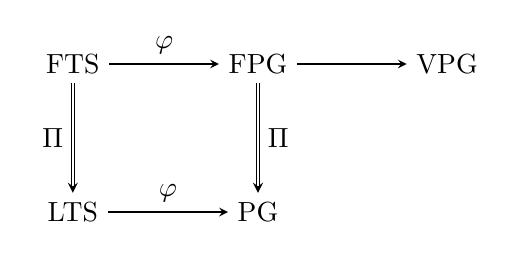
\begin{tikzpicture}
\matrix (m) [matrix of math nodes,row sep=4em,column sep=4em,minimum width=2em]
{
	\text{FTS} & \text{FPG} & \text{VPG} \\
	\text{LTS} & \text{PG} \\};
\path[-stealth]
(m-1-1) edge [double] node [left] {$\Pi$} (m-2-1)
edge node [above] {$\varphi$} (m-1-2)
(m-2-1.east|-m-2-2) edge node [above] {$\varphi$}
(m-2-2)
(m-1-2) edge [double] node [right] {$\Pi$} (m-2-2)
edge (m-1-3);
\end{tikzpicture}\\
Finally we show that solving VPGs, ie. finding the winning sets for all configurations, can be used to verify FTSs.
\begin{theorem}
	\label{the_VPG_ver_FTS}
	Given:
	\begin{itemize}
		\item FTS $M = (S, Act, trans, s_0, N, P, \gamma)$,
		\item closed modal mu-calculus formula $\varphi$,
		\item product $p \in P$ and
		\item state $s \in S$
	\end{itemize}
	it holds that $(M_{|p}, s) \models \varphi$ if and only if $(s, \varphi) \in W_0^{p}$ in $\textit{FPG2VPG}(\textit{FTS2FPG}(M, \varphi))$.
	\begin{proof}
		Let $W_0^{p}$ and $W_1^{p}$ denote the winning sets for game $\textit{FPG2VPG}(\textit{FTS2FPG}(M, \varphi))$. And $Q_0^{p}$ and $Q_1^{p}$ denote the winning sets for game $\textit{FTS2FPG}(M, \varphi)$.
		
		Using theorem \ref{the_FPG_ver_FTS} we find that $(M_{|p}, s) \models \varphi$ if and only if $(s, \varphi) \in Q_0^{p}$. If $(s, \varphi) \in Q_0^{p}$ then we find by using theorem \ref{the_FPG_sub_VPG} that $(s, \varphi) \in W_0^{p}$. If $(s, \varphi) \not\in Q_0^{p}$ then $(s, \varphi) \in Q_1^{p}$ and therefore $(s, \varphi) \in W_1^{p}$ and $(s, \varphi) \not\in W_0^{p}$.
	\end{proof}
\end{theorem}
Using this theorem we can visualize verification of an FTS in figure \ref{fig:ftsverificationusingvpg}.
\begin{figure}[h]
	\centering
	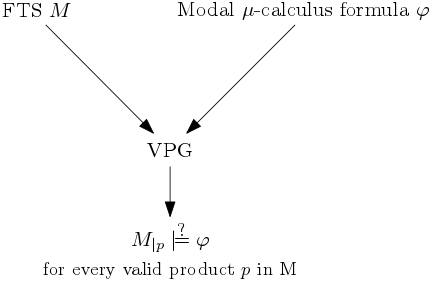
\includegraphics[scale=0.5]{Diagrams/FTSVerificationUsingVPG}
	\caption[FTS verification using VPG]{FTS verification using VPG}
	\label{fig:ftsverificationusingvpg}
\end{figure}

\pagebreak
\section{Solving variability parity games}
For solving VPGs we distinguish two general approaches, the first approach is to simply project the VPG to the different configurations and solve all the resulting parity games independently. We call this approach \textit{product} based. Alternatively we solve the VPG \textit{family} based where a VPG is solved in its entirety and similarities are used to improve performance. 

In this next sections we explore family based algorithms, analyse their running time complexity and present the results of experiments conducted to test the performance of the different family based algorithms compared to the product based approach.

In general we can take some existing algorithm to solve parity games with running time complexity $O(T)$ and use the algorithm to solve a VPG product based. For a VPG with configurations $\mathfrak{C}$ this gives a running time complexity of $O(|\mathfrak{C}|T)$.


\subsection{Preliminaries}
\section{Fixed-point theory} 
A fixed-point of a function is an element in the domain of that function such that the function maps to itself for that element. Fixed-points are used in model verification as well as in some parity game algorithms.

Fixed-point theory goes hand in hand with lattice theory which we introduce first.
\subsection{Lattices}
We introduce definitions for ordering and lattices taken from \cite{birkhoff1940lattice}.
\begin{definition}[\cite{birkhoff1940lattice}]
	A partial order is a binary relation $x \leq y$ on set $S$ where for all $x,y,z \in S$ we have:
	\begin{itemize}
		\item $x \leq x$. (Reflexive)
		\item If $x \leq y$ and $y \leq x$, then $x=y$. (Antisymmetric)
		\item If $x \leq y$ and $y \leq z$, then $x \leq z$. (Transitive)
	\end{itemize}
\end{definition}

\begin{definition}[\cite{birkhoff1940lattice}]
	A partially ordered set is a set $S$ and a partial order $\leq$ for that set, we denote a partially ordered set by $\langle S, \leq \rangle$.
\end{definition}

\begin{definition}[\cite{birkhoff1940lattice}]
	Given partially ordered set $\langle P,\leq \rangle$ and subset $X \subseteq P$. An upper bound to $X$ is an element $a \in P$ such that $x \leq a$ for every $x\in X$. A least upper bound to $X$ is an upper bound $a \in P$ such every other upper bound is larger or equal to $a$.
\end{definition}
The term least upper bound is synonymous with the term supremum, we write $\sup \{ S \}$ to denote the supremum of set $S$.
\begin{definition}[\cite{birkhoff1940lattice}]
	Given partially ordered set $\langle P,\leq \rangle$ and subset $X \subseteq P$. A lower bound to $X$ is an element $a \in P$ such that $a \leq x$ for every $x\in X$. A greatest lower bound to $X$ is a lower bound $a \in P$ such that every other lower bound is smaller or equal to $a$.
\end{definition}
The term greatest lower bound is synonymous with the term infimum, we write $\inf \{ S\}$ to denote the infimum of set $S$.

\begin{definition}[\cite{birkhoff1940lattice}]
	A lattice is a partially ordered set where any two of its elements have a supremum and an infimum.
\end{definition}

\begin{definition}[\cite{birkhoff1940lattice}]
	A complete lattice is a partially ordered set in which every subset has a supremum and an infimum.
\end{definition}

\begin{definition}[\cite{birkhoff1940lattice}]
	Given a lattice $\langle D, \leq \rangle$, function $f : D \rightarrow D$ is monotonic if for all $x \in D$ and $y \in D$ it holds that if $x \leq y$ then $f(x) \leq f(y)$.
\end{definition}
\subsection{Fixed-points}
Fixed-points are formally defined as follows:
\begin{definition}
	Given function $f : D \rightarrow D$ the value $x \in D$ is a fixed-point for $f$ if and only if $f(x) = x$. Furthermore $x$ is the least fixed-point for $f$ if every other fixed-point for $f$ is greater or equal to $x$ and dually $x$ is the greatest fixed-point for $f$ if every other fixed-point $f$ is less or equal to $x$.
\end{definition}
The Knaster-Tarski theorem states that least and greatest fixed-points exist for some domain and function given that a few conditions hold.
The theorem, as written down by Tarski in \cite{tarski1955}, states:
\begin{theorem}[Knaster-Tarski\cite{tarski1955}]
	\label{the_knaster_tarski}
	Let
	\begin{itemize}
		\item $\langle A, \leq \rangle$ be a complete lattice,
		\item $f$ be a monotonic function on $A$ to $A$,
		\item $P$ be the set of all fixpoints of f.
	\end{itemize}
	Then the set $P$ is not empty and the system $\langle P, \leq \rangle$ is a complete lattice; in particular we have 
	\[ \sup P = \sup \{ x\ |\ f(x) \geq x \} \in P \]
	and
	\[ \inf P = \inf \{ x\ |\ f(x) \leq x \} \in P \]
\end{theorem}

\section{Model verification}
It is difficult to develop correct software, one way to improve reliability of software is through model verification; the behaviour of software is specified in a model and formal verification techniques are used to show that the behaviour adheres to certain requirements. In this section we inspect how to model behaviour and how to specify requirements.

Behaviour can be modelled as a \textit{labelled transition system} (LTS). An LTS consists of states in which the system can find itself and transitions between states. Transitions represent the possible state change of the system. Transitions are labelled with actions that indicate what kind of change is happening. Formally we define an LTS as follows.
\begin{definition}[\cite{Groote}]
	\label{def_lts}
	A labelled transition system (LTS) is a tuple $M = (S, Act, trans, s_0)$, where:
	\begin{itemize}
		\item $S$ is a finite set of states,
		\item $Act$ a finite set of actions,
		\item $trans \subseteq S \times Act \times S$ is the transition relation with $(s,a,s') \in trans$ denoted by $s \xrightarrow a s'$,
		\item $s_0 \in S$ is the initial state.
	\end{itemize}
\end{definition}

An LTS is usually depicted as a graph where the vertices represent the states, the edges represent the transitions, edges are labelled with actions and an edge with no origin vertex indicates the initial state. Such a representation is depicted in the example below.
\begin{example}[\cite{FamBasedModelCheckingWithMCRL2}]
	Consider the behaviour of a coffee machine that accepts a coin after which it serves a standard coffee, this can be repeated infinitely often. 
	
	The behaviour can be modelled as an LTS that has two states: in the initial state it is ready to accept a coin and in the second state it is ready to serve a standard coffee. We introduce two actions: \textit{ins}, which represents a coin being inserted, and \textit{std}, which represents a standard coffee being served. We get the following LTS which is also depicted in Figure \ref{fig:coffeemachinebasiceurolts}.
	\[ (\{s_1,s_2\},\{std,ins\},\{(s_1,ins,s_2),(s_2,std,s_1)\},s_1)\]
	\begin{figure}[h]
		\centering
		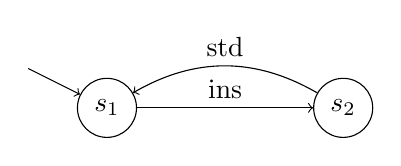
\begin{tikzpicture}[->]
			\tikzstyle{state} = [circle,draw,minimum size=0.75cm]
			
			\node[state] (s1) at (1,0) {$s_1$};
			\node[state] (s2) at (4,0) {$s_2$};
			
			\path (s1) edge node[above]{ins} (s2) ;
			\path (s2) edge[bend right] node[above]{std} (s1) ;
			\path (0,0.5) edge (s1);
		\end{tikzpicture}
		\caption[Coffee machine LTS]{Coffee machine LTS $C$}
		\label{fig:coffeemachinebasiceurolts}
	\end{figure}
\end{example}

LTSs might be non-deterministic, meaning that from a state there might be multiple transitions that can be taken, moreover multiple transitions with the same action can be taken. This is depicted in the example below.

\begin{example}
	We extend the coffee machine example where at some point the coffee machine can be empty and needs a fill before the system is ready to receive a coin again. This LTS is depicted in Figure \ref{fig:coffeemachineundeterministic}. When the \textit{std} transition is taken from state $s_2$ it is non-determined in which states the system ends.
	\begin{figure}[h]
		\centering
		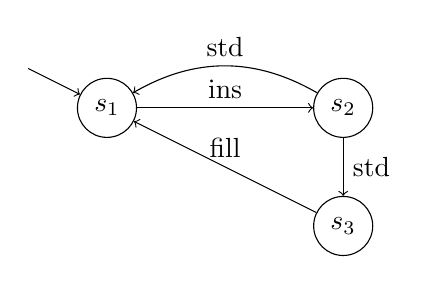
\begin{tikzpicture}[->]
			\tikzstyle{state} = [circle,draw,minimum size=0.75cm]
			
			\node[state] (s1) at (1,1.5) {$s_1$};
			\node[state] (s2) at (4,1.5) {$s_2$};
			\node[state] (s3) at (4,0) {$s_3$};
			
			\path (s1) edge node[above]{ins} (s2) ;
			\path (s2) edge[bend right] node[above]{std} (s1) ;
			\path (s2) edge node [right]{std} (s3);
			\path (s3) edge node [above]{fill} (s1);
			\path (0,2) edge (s1);
		\end{tikzpicture}
		\caption[Coffee machine LTS]{Coffee machine with non-deterministic behaviour}
		\label{fig:coffeemachineundeterministic}
	\end{figure}
\end{example}


A system can be verified by checking if its behaviour adheres to certain requirements. The behaviour can be modelled in an LTS. Requirements can be expressed in a temporal logic; with a temporal logic we can express certain propositions with a time constraint such as \textit{always}, \textit{never} or \textit{eventually}. For example (relating to the coffee machine example) we can express the following constraint: "After a coin is inserted the machine always serves a standard coffee immediately afterwards". The most expressive temporal logic is the modal $\mu$-calculus. A modal $\mu$-calculus formula is expressed over a set of actions and a set of variables.

We define the syntax of the modal $\mu$-calculus below. Note that the syntax is in positive normal form, ie. no negations.
\begin{definition}[\cite{Groote}]
	\label{def_mu_syntax}
	A modal $\mu$-calculus formula over the set of actions $Act$ and a set of variables $\mathcal{X}$ is defined by
	\[ \varphi = \top\ |\ \bot\ |\ X\ |\ \varphi \vee \varphi\ |\ \varphi \wedge \varphi\ |\ \langle a \rangle \varphi\ |\ [a]\varphi\ |\ \mu X.\varphi\ |\ \nu X.\varphi \]
	with $a \in Act$ and $X \in \mathcal{X}$. 
\end{definition}
The modal $\mu$-calculus contains boolean constants $\top$ and $\bot$, propositional operators $\vee$ and $\wedge$, modal operators $\langle \, \rangle$ and $[ \, ]$ and fixpoint operators $\mu$ and $\nu$. 

A variable $X \in \mathcal{X}$ \textit{occurs free} in formula $\phi$ if and only if $X$ occurs in $\phi$ such that $X$ is not a sub-formula of $\mu X.\phi'$ or $\nu X.\phi'$ in $\phi$. A formula is \textit{closed} if and only if there are no variables that occurs free.

A formula can be interpreted in the context of an LTS, such an interpretation results in a set of states in which the formula holds. Given formula $\varphi$ we define the interpretation of $\varphi$ as $\llbracket \varphi \rrbracket ^\eta  \subseteq S$ where $\eta : \mathcal{X}\rightarrow 2^S$ maps a variable to a set of states. We can assign $S' \subseteq S$ to variable $X$ in $\eta$ by writing $\eta[X:=S']$, ie. $(\eta[X:=S'])(X) = S'$.
\begin{definition}
	\label{def_mu_sem} For LTS $(S, Act, trans, s_0)$ we inductively define the interpretation of a modal $\mu$-calculus formula $\varphi$, notation
	$\llbracket \varphi \rrbracket^\eta$, where $\eta : \mathcal{X} \rightarrow \mathcal{P}(S)$ is a variable valuation, as a set of states
	where $\varphi$ is valid, by:
	\begin{align*}
	&\llbracket {\top} \rrbracket^\eta &&= S\\
	&\llbracket {\bot} \rrbracket^\eta &&= \emptyset\\
	&\llbracket \varphi_1 \wedge \varphi_2 \rrbracket^\eta &&= \llbracket \varphi_1 \rrbracket^\eta \cap \llbracket \varphi_2 \rrbracket^\eta \\
	&\llbracket \varphi_1 \vee \varphi_2 \rrbracket^\eta &&= \llbracket \varphi_1 \rrbracket^\eta \cup \llbracket \varphi_2 \rrbracket^\eta\\
	&\llbracket \langle a \rangle \varphi \rrbracket^\eta &&= \{s \in S|\exists_{s' \in S}\ s \xrightarrow {a} s' \wedge s' \in \llbracket \varphi \rrbracket^\eta\}\\
	&\llbracket [ a ] \varphi \rrbracket^\eta &&= \{s \in S|\forall_{s' \in S}\ s \xrightarrow {a} s' \implies s' \in \llbracket \varphi \rrbracket^\eta\}\\
	&\llbracket \mu X. \varphi \rrbracket^\eta &&= \bigcap\{f \subseteq S | f \supseteq \llbracket \varphi \rrbracket^{\eta[X:=f]}\}\\
	&\llbracket \nu X. \varphi \rrbracket^\eta &&= \bigcup\{f \subseteq S | f \subseteq \llbracket \varphi \rrbracket^{\eta[X:=f]}\}\\
	&\llbracket X \rrbracket^\eta &&= \eta(X)
	\end{align*}
\end{definition}
Since there are no negations in the syntax we find that every modal $\mu$-calculus formula is monotone, ie. if we have for $U \subseteq S$ and $U' \subseteq S$ that $U \subseteq U'$ holds then $\llbracket \varphi \rrbracket^{\eta[X:=U]} \subseteq \llbracket \varphi \rrbracket^{\eta[X:=U']}$ holds for any variable $X \in \mathcal{X}$. Using the Knaster-Tarski theorem (Theorem \ref{the_knaster_tarski}) we find that the least and greatest fixed-points always exist.

Given closed formula $\varphi$, LTS $M = (S, Act, trans, s_0)$ and $s \in S$ we say that $M$ satisfies formula $\varphi$ in state $s$, and write $(M,s) \models \varphi$, if and only if $s \in \llbracket \varphi \rrbracket^\eta$. If and only if $M$ satisfies $\varphi$ in the initial state do we say that $M$ satisfies formula $\varphi$ and write $M \models \varphi$. 

\begin{example}[\cite{FamBasedModelCheckingWithMCRL2}]
	Consider the coffee machine example from Figure \ref{fig:coffeemachinebasiceurolts} and formula $\varphi = \nu X. \mu Y([inst]Y \wedge [std]X)$ which states that action \textit{std} must occur infinitely often over all infinite runs. Obviously this holds for the coffee machine, therefore we have $C \models \varphi$.
\end{example}

\section{Parity games}
A \textit{parity game} is a game played by two players: player 0 (also called player \textit{even}) and player 1 (also called player \textit{odd}). We write $\alpha \in \{0,1\}$ to denote an arbitrary player and $\overline{\alpha}$ to denote $\alpha$'s opponent, ie. $\overline{0} = 1$ and $\overline{1} = 0$. A parity game is played on a playing field which is a directed graph where every vertex is owned by either player 0 or player 1. Furthermore every vertex has a natural number, called its \textit{priority}, associated with it.
\begin{definition}[\cite{Bradfield2018}]
	\label{def_PG}
	A parity game is a tuple $(V, V_0, V_1, E, \Omega)$, where:
	\begin{itemize}
		\item $V$ is a finite set of vertices partitioned in sets $V_0$ and $V_1$, containing vertices owned by player 0 and player 1 respectively,
		\item $E \subseteq V \times V$ is the edge relation,
		\item $\Omega :  V \rightarrow \mathbb{N}$ is the priority assignment function.
	\end{itemize}
\end{definition}
Parity games are usually represented as a graph where vertices owned by player 0 are shown as diamonds and vertices owned by player 1 are shown as boxes, furthermore the priorities are depicted as numbers inside the vertices. Such a representation is shown in the example below.

\begin{example}
	Figure \ref{fig:simplepgpg} shows the parity game:
	\[ V_0 = \{v_1,v_4,v_5\},V_1 = \{v_2,v_3\}, V = V_0 \cup V_1\]
	\[ E = \{(v_1,v_2),(v_2,v_1),(v_1,v_3),(v_2,v_4),(v_3,v_4),(v_3,v_5),(v_4,v_4)\}\] 
	\[ \Omega = \{v_1 \mapsto 2, v_2 \mapsto 3, v_3 \mapsto 0, v_4 \mapsto 0, v_5 \mapsto 1 \}\]
	\begin{figure}[h]
		\centering
		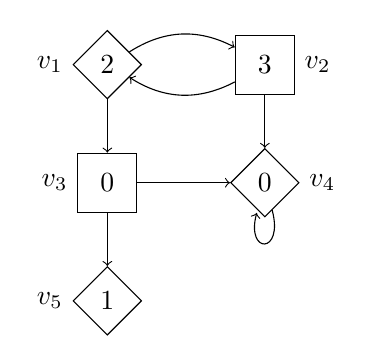
\begin{tikzpicture}[->]
			\tikzstyle{even} = [diamond,draw,minimum size=0.75cm]
			\tikzstyle{odd}  = [rectangle,draw,shape aspect=1,minimum size=0.75cm]
			
			\node[even,label=west:$v_1$] (v1) at (0,3) {2};
			\node[odd, label=east:$v_2$] (v2) at (2,3) {3};
			\node[odd, label=west:$v_3$] (v3) at (0,1.5) {0};
			\node[even,label=east:$v_4$] (v4) at (2,1.5) {0};
			\node[even,label=west:$v_5$] (v5) at (0,0) {1};
			
			\path (v3) edge (v5) ;
			\path (v1) edge [bend left] (v2) ;
			\path (v2) edge [bend left] (v1) ;
			\path (v1) edge (v3) ;
			\path (v3) edge (v4) ;
			\path (v2) edge (v4) ;
			\path (v4) edge [loop below] (v4);
		\end{tikzpicture}
		\caption[Parity game example]{Parity game example}
		\label{fig:simplepgpg}
	\end{figure}
\end{example}

A parity game can be played for a vertex $v \in V$. We start by placing a token on vertex $v$, the player that owns vertex $v$ can choose to move the token along an edge to a vertex $w \in V$ such that $(v,w) \in E$. Again the player that owns vertex $w$ can choose where to move the token next. This is repeated either infinitely often or until a player cannot make a move, ie. the token is on a vertex with no outgoing edges. Playing in this manner gives a sequence of vertices, called a \textit{path}, starting from vertex $v$. For path $\pi$ we write $\pi_i$ to denote $i^\text{th}$ vertex in path $\pi$. Every path is associated with a winner (either player 0 or 1). If a player $\alpha$ cannot move at some point we get a finite path and player $\overline{\alpha}$ wins the path. If we get an infinite path $\pi$ then the winner is determined by the parity of the highest priority that occurs infinitely often in the path. Formally we determine the highest priority occurring infinitely often by the following formula.
\[ \max\{ p \ |\ \forall_j \exists_i j < i \wedge p = \Omega(\pi_i) \}\] 
If the highest priority is odd then player $1$ wins the path, if it is even player $0$ wins the path.

A path is \textit{valid} if and only if for every $i > 0$ such that $\pi_i$ exists we have $(\pi_{i-1},\pi_i) \in E$.


\begin{example}
	Again consider the example in Figure \ref{fig:simplepgpg}. If we play the game for vertex $v_1$ we start by placing a token on $v_1$. Consider the following exemplary paths where $(w_1{\dots}w_m)^\omega$ indicates an infinite repetition of vertices $w_1{\dots}w_m$.
	\begin{itemize}
		\item $\pi = v_1v_3v_5$ is won by player $1$ since player $0$ cannot move at $v_5$.
		\item $\pi = (v_1v_2)^\omega$ is won by player $1$ since the highest priority occurring infinitely often is 3.
		\item $\pi = v_1v_3(v_4)^\omega$ is won by player $0$ since the highest priority occurring infinitely often is $0$.
	\end{itemize}
\end{example}

The moves that the players make are determined by their \textit{strategies}. A strategy $\sigma_\alpha$ determines for a vertex in $V_\alpha$ where the token goes next. We can define a strategy for player $\alpha$ as a partial function $\sigma_\alpha : V^*V_\alpha \rightarrow V$ that maps a series of vertices ending with a vertex owned by player $\alpha$ to the next vertex such that for any $\sigma_\alpha(w_0\dots w_m) = w$ we have $(w_m,w) \in E$. A path $\pi$ \textit{conforms to} strategy $\sigma_\alpha$ if for every $i > 0$ such that $\pi_i$ exists and $\pi_{i-1} \in V_\alpha$ we have $\pi_i = \sigma_\alpha(\pi_0\pi_1\dots\pi_{i-1})$.

A strategy is \textit{winning} for player $\alpha$ from vertex $v$ if and only if $\alpha$ is the winner of every valid path starting in $v$ that conforms to $\sigma_\alpha$. If such a strategy exists for player $\alpha$ from vertex $v$ we say that vertex $v$ is winning for player $\alpha$.

\begin{example}
	In the parity game seen in Figure \ref{fig:simplepgpg} vertex $v_1$ is winning for player 1. Player 1 has a strategy that plays every vertex sequence ending in $v_2$ to $v_1$ and plays every vertex sequence ending in $v_3$ to $v_5$. Regardless of the strategy for player 0 the path will either end up in $v_5$ or will pass $v_2$ infinitely often. In the former case player 1 wins the path because player 0 can not move at $v_5$. In the latter case the highest priority occurring infinitely often is 3.
\end{example}

Parity games are known to be positionally determined \cite{Bradfield2018}, meaning that every vertex in a parity game is winning for one of the two players. Also every player has a \textit{positional strategy} that is winning starting from each of his/her winning vertices. A positional strategy is a strategy that only takes the current vertex into account to determine the next vertex, it does not look at already visited vertices. Therefore we can consider a strategy for player $\alpha$ as a complete functions $\sigma_\alpha : V_\alpha \rightarrow V$. Finally it is decidable for each of the vertices in a parity who the winner is \cite{Bradfield2018}.

A parity game is \textit{solved} if the vertices are partitioned in two sets, namely $W_0$ and $W_1$, such that every vertex in $W_0$ is winning for player 0 and every vertex in $W_1$ is winning for player 1. We call these sets the \textit{winning sets} of a parity game.

Finally parity games are considered \textit{total} if and only if every vertex has at least one outgoing edge. Playing a total parity game always results in an infinite path. We can make a non-total parity game total by adding two sink vertices: $l_0$ and $l_1$. Each sink vertex has only one outgoing edge, namely to itself. Vertex $l_0$ has priority 1 and vertex $l_1$ has priority 0. Clearly if the token ends up in $l_\alpha$ then player $\alpha$ looses the game because with only one outgoing edge we only get a single priority that occurs infinitely often, namely priority $\overline{\alpha}$. For every vertex $v \in V_\alpha$ that does not have an outgoing edge we create an edge from $v$ to $l_\alpha$. In the original game player $\alpha$ lost when the token was in vertex $v$ because he/she could not move any more. In the total game player $\alpha$ can only play to $l_\alpha$ from $v$ where he/she still looses. So using this method vertices in the total game have the same winner as they had in the original game (except for $l_0$ and $l_1$ which did not exist in the original game). In general we try to only work with total games because no distinction is required between finite paths and infinite paths when reasoning about them, however we will encounter some scenario's where non-total games are still considered.

\subsection{Relation between parity games and model checking}
Verifying LTSs against a modal $\mu$-calculus formula can be done by solving a parity game. This is done by translating an LTS in combination with a formula to a parity game, the solution of the parity game provides the information needed to conclude if the model satisfies the formula. This relation is depicted in Figure \ref{fig:ltsverificationusingpg}. 
\begin{figure}[h]
	\centering
	\begin{tikzpicture}[->]
		\tikzstyle{even} = [diamond,draw,minimum size=0.75cm]
		\tikzstyle{odd}  = [rectangle,draw,shape aspect=1,minimum size=0.75cm]
		
		\node (lts) at (0,5)  {LTS $M$};
		\node (form)at (6,5)  {Modal $\mu$-calculus formula $\varphi$};
		\node (PG)  at (3,2.5){PG};
		\node (check)at (3,0){$M \stackrel{?}{\models} \varphi$};
		
		\path (lts) edge (PG);
		\path (form)edge (PG);
		\path (PG)  edge (check);
	\end{tikzpicture}
	\caption[LTS verification using PG]{LTS verification using PG}
	\label{fig:ltsverificationusingpg}
\end{figure}

We consider a method of creating parity games from an LTS and a modal $\mu$-calculus formula such that there is a special vertex $w$ in the parity game that indicates if the LTS satisfies the formula; if and only if $w$ is won by player 0 is the formula satisfied.

First we introduce the notion of unfolding. A fixpoint formula $\mu X . \varphi$ can be unfolded, resulting in formula $\varphi$ where every occurrence of $X$ is replaced by $\mu X . \varphi$, denoted by $\varphi [ X:= \mu X . \varphi]$. Interpreting a fixpoint formula results in the same set as interpreting its unfolding as shown in \cite{Bradfield2018}; i.e. $[\![\mu X . \varphi]\!]^\eta = [\![\varphi[X:=\mu X . \varphi]]\!]^\eta$. The same holds for the fixpoint operator $\nu$.

Next we define the Fischer-Ladner closure for a closed $\mu$-calculus formula 
\cite{STREETT1989249,FISCHER1979194}. The Fischer-Ladner closure of $\varphi$ is the set $\textit{FL}(\varphi)$ of closed formulas containing at least $\varphi$. Furthermore for every formula $\psi$ in $\textit{FL}(\varphi)$ it holds that for every direct subformula $\psi'$ of $\psi$ there is a formula in $\textit{FL}(\varphi)$ that is equivalent to $\psi'$.
\begin{definition}
	\label{def_FLClosure}
	The Fischer-Ladner closure of closed $\mu$-calculus formula $\varphi$ is the smallest set $\textit{FL}(\varphi)$ satisfying the following constraints:
	\begin{itemize}
		\item $\varphi \in \textit{FL}(\varphi)$,
		\item if $\varphi_1 \vee \varphi_2 \in \textit{FL}(\varphi)$ then $\varphi_1 ,\varphi_2 \in \textit{FL}(\varphi)$,
		\item if $\varphi_1 \wedge \varphi_2 \in \textit{FL}(\varphi)$ then $\varphi_1 ,\varphi_2 \in \textit{FL}(\varphi)$,
		\item if $\langle a \rangle \varphi' \in \textit{FL}(\varphi)$ then $\varphi' \in \textit{FL}(\varphi)$,
		\item if $[ a ] \varphi' \in \textit{FL}(\varphi)$ then $\varphi' \in \textit{FL}(\varphi)$,
		\item if $\mu X . \varphi' \in \textit{FL}(\varphi)$ then $\varphi'[X:= \mu X . \varphi'] \in \textit{FL}(\varphi)$ and
		\item if $\nu X . \varphi' \in \textit{FL}(\varphi)$ then $\varphi'[X:= \nu X . \varphi'] \in \textit{FL}(\varphi)$.
		
	\end{itemize}
\end{definition}

We also define the alternation depth of a formula.
\begin{definition}[\cite{Bradfield2018}]
	The dependency order on bound variables of $\varphi$	is the smallest partial order such that $X \leq_\varphi Y$ if $X$ occurs free in $\sigma Y. \psi$ . The alternation depth of a $\mu$-variable X in formula $\varphi $ is the maximal length of a chain $X_1 \leq_\varphi  \dots \leq_\varphi X_n$ where $X = X_1$, variables $X_1, X_3, \dots$ are $\mu$-variables and variables $X_2, X_4, \dots$ are $\nu$-variables. The alternation depth of a $\nu$-variable is defined similarly. The alternation depth of formula $\varphi$, denoted $adepth(\varphi)$, is the maximum of the alternation depths of the variables bound in $\varphi$, or zero if there are no fixpoints.
\end{definition}
\begin{example}
	Consider the formula $\varphi = \nu X. \mu Y. ([ins]Y \wedge [std] X)$ which states that for an LTS with $Act = \{ ins, std\}$ the action \textit{std} must occur infinitely often over all infinite runs. Since $X$ occurs free in $\mu Y. ([ins] Y \wedge [std]X)$ we have $adepth(Y) = 1$ and $adepth(X) = 2$.
\end{example}
As shown in \cite{Bradfield2018} it holds that formula $\mu X. \psi$ has the same alternation depth as its unfolding $\psi[X:=\mu X. \psi]$. Similarly for the greatest fixpoint. 

Next we define the transformation from an LTS and a formula to a parity game.
\begin{definition}[\cite{Bradfield2018}]
	\label{def_LTS2PG}
	LTS2PG($M, \varphi$) converts LTS $M = (S, Act, trans, s_0)$ and closed formula $\varphi$ to a parity game $(V, V_0, V_1, E, \Omega)$.
	
	Vertices in the parity game are presented as pairs of states and sub-formulas. A vertex is created for every state with every formula in the Fischer-Ladner closure of $\varphi$. We define the set of vertices:
	\[ V = S \times \textit{FL}(\varphi) \]
	
	Vertices have the following owners, successors and priorities:\\
	\begin{center}
		\begin{tabular}{l|l|l|l}
			Vertex & Owner & Successor(s) & Priority \\\hline
			$(s,\bot)$ & 0     &       & 0 \\
			$(s,\top)$ & 1     &      & 0 \\
			$(s,\psi_1 \vee \psi_2)$ & 0       & $(s,\psi_1)$ and $(s,\psi_2)$  & 0 \\
			$(s,\psi_1 \wedge \psi_2)$ & 1       & $(s,\psi_1)$ and $(s,\psi_2)$  & 0 \\
			$(s, \langle a \rangle \psi)$ & 0 & $(s',\psi)$ for every $s \xrightarrow{ a} s'$  & 0 \\
			$(s, [ a ] \psi)$ & 1 & $(s',\psi)$ for every $s \xrightarrow{ a} s'$ & 0 \\
			$(s, \mu X. \psi)$ & 1 & $(s, \psi[X:= \mu X. \psi])$ & $2 \lfloor adepth(X) / 2 \rfloor + 1$ \\
			$(s, \nu X. \psi)$ & 1 & $(s, \psi[X:= \nu X. \psi])$ & $2 \lfloor adepth(X) / 2 \rfloor$
		\end{tabular}
	\end{center}

	Since the Fischer-Ladner formula's are closed we never get a vertex $(s,X)$.
\end{definition}
\begin{example}
	Consider LTS $M$ in Figure \ref{fig:exverltsprojempty} and formula $\varphi = \mu X.([a]X \vee \langle b \rangle \top)$ expressing that on any path reached by $a$'s we can eventually do a $b$ action.
	\begin{figure}[h]
		\centering
		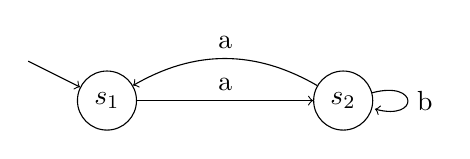
\begin{tikzpicture}[->]
			\tikzstyle{state} = [circle,draw,minimum size=0.75cm]
			
			\node[state] (s1) at (1,1.5) {$s_1$};
			\node[state] (s2) at (4,1.5) {$s_2$};
			
			\path (s1) edge node[above]{a} (s2) ;
			\path (s2) edge[bend right] node[above]{a} (s1) ;
			\path (s2) edge [loop right] node[right]{b} (s2);
			
			\path (0,2) edge (s1);
		\end{tikzpicture}
		\caption[LTS $M$]{LTS $M$}
		\label{fig:exverltsprojempty}
	\end{figure}

	The resulting parity game is depicted in Figure \ref{fig:exverpg}. Let $V$ denote the set of vertices of this parity game. There are two vertices with more than one outgoing edge. From vertex $(s_1, [a](\mu X.\phi) \vee \langle b \rangle \top)$ player 0 does not want to play to $(s_1, \langle b \rangle \top)$ because he/she will not be able to make another move and looses the path. From vertex $(s_2, [a](\mu X.\phi)  \vee \langle b \rangle \top)$ player 0 can play to $(s_2, \langle b \rangle \top)$ to bring the play in $(s_2,\top)$ to win the path. We get the following winning sets:
	\begin{align*}
	W_1 &= \{ (s_1, \langle b \rangle \top )\}\\
	W_0 &= V \backslash W_1
	\end{align*}
	With the strategies $\sigma_0$ for player $0$ and $\sigma_1$ for player $1$ being (vertices with one outgoing edge are omitted):
	\begin{align*}
	\sigma_0 = \{
	&(s_1, [a](\mu X. \phi) \vee \langle b \rangle \top) \mapsto (s_1, [a] (\mu X. \phi)), \\
	&(s_2, [a](\mu X. \phi) \vee \langle b \rangle \top) \mapsto (s_2, \langle b \rangle \top) \} \\
	\sigma_1 = \{&\}
	\end{align*}
	Note that the choice where to go from $(s_2, [a](\mu X.\phi) \vee \langle b \rangle \top)$ does not matter for the winning sets.
	\begin{figure}[h]
		\centering
		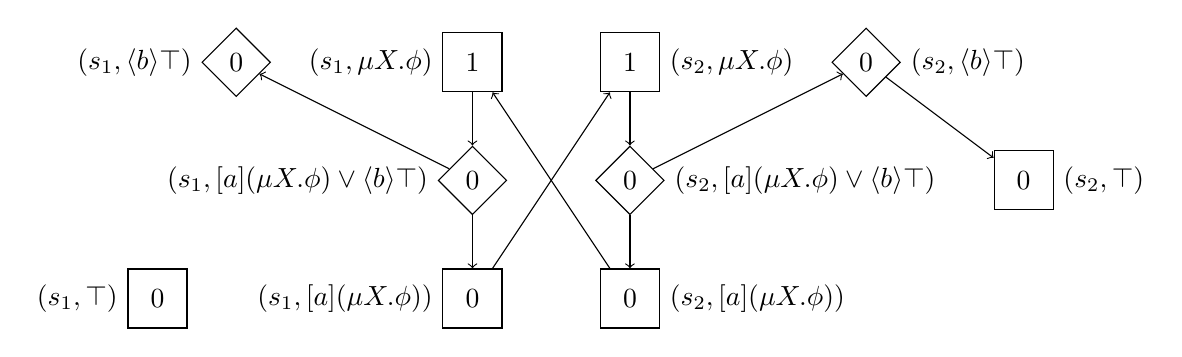
\begin{tikzpicture}[->]
			\tikzstyle{even} = [diamond,draw,minimum size=0.75cm]
			\tikzstyle{odd}  = [rectangle,draw,shape aspect=1,minimum size=0.75cm]
			
			\node[even,label={west:$(s_1,\langle b \rangle\top)$}] (s1<b>T) at (10,10) {0};
			\node[odd,label={west:$(s_1,\top)$}] (s1T) at (9,7) {0};
			
			
			\node[odd,label={west:$(s_1,\mu X.\phi)$}] (s1muxphi) at (13,10) {1};
			\node[even,label={west:$(s_1,[a](\mu X.\phi) \vee \langle b \rangle \top)$}] (s1muxphiunf) at (13,8.5) {0};
			\node[odd,label={west:$(s_1,[a](\mu X .\phi))$}] (s1[a]muxphi) at (13,7) {0};
			
			\node[odd,label={east:$(s_2,\mu X.\phi)$}] (s2muxphi) at (15,10) {1};
			\node[even,label={east:$(s_2,[a](\mu X.\phi) \vee \langle b \rangle \top)$}] (s2muxphiunf) at (15,8.5) {0};
			\node[odd,label={east:$(s_2,[a](\mu X .\phi))$}] (s2[a]muxphi) at (15,7) {0};
			
			
			\node[even,label={east:$(s_2,\langle b \rangle\top)$}] (s2<b>T) at (18,10) {0};
			\node[odd,label={east:$(s_2,\top)$}] (s2T) at (20,8.5) {0};
			
			\path (s1muxphiunf) edge (s1<b>T);
			\path (s1muxphi) edge (s1muxphiunf);
			\path (s1muxphiunf) edge (s1[a]muxphi);
			
			\path (s2muxphiunf) edge (s2<b>T);
			\path (s2muxphi) edge (s2muxphiunf);
			\path (s2muxphiunf) edge (s2[a]muxphi);
			\path (s2<b>T) edge (s2T);
			
			\path(s1[a]muxphi) edge (s2muxphi);
			\path(s2[a]muxphi) edge (s1muxphi);
		\end{tikzpicture}
		
		\caption[Parity game $LTS2PG(M, \varphi)$]{Parity game $LTS2PG(M, \varphi)$ with $\phi = [a] X \vee \langle b \rangle \top$}
		\label{fig:exverpg}
	\end{figure}
\end{example}

Parity games created in this manner relate back to the model verification question; state $s$ in LTS $M$ satisfies $\varphi$ if and only if player $0$ wins vertex $(s, \varphi)$. This is formally stated in the following theorem which is proven in \cite{Bradfield2018}.
\begin{theorem}[\cite{Bradfield2018}]
	\label{the_LTS_PG_REL}Given LTS $M = (S, Act, trans, s_0)$, modal $\mu$-calculus formula $\varphi$ and state $s \in S$ it holds that $(M, s) \models \varphi$ if and only if $(s,\varphi) \in W_0$ for the game $LTS2PG(M, \varphi)$.
\end{theorem}

\subsection{Globally and locally solving parity games}
Parity games can be solved \textit{globally} or \textit{locally}; globally solving a parity game means that for every vertex in the game it is determined who the winner is. Locally solving a parity game means that for a specific vertex in the game it is determined who the winner is. For some applications of parity games, including model checking, there is a specific vertex that needs to be solved to solve the original problem. Locally solving the parity game is sufficient in such cases to solve the original problem.

Most parity game algorithms (including the two considered next) are concerned with globally solving, when talking about solving a parity game we talk about globally solving it unless stated otherwise. 

\subsection{Parity game algorithms}
Various algorithms for solving parity games are known, we introduce two of them. First Zielonka's recursive algorithm which is well studied and generally considered to be one of the best performing parity game algorithms in practice \cite{Oink,SolvingPGInPractice}. We also inspect the fixed-point iteration algorithm which tends to perform well for model-checking problems with a low number of distinct priorities \cite{BDDSolvingPG}.

\subsubsection{Zielonka's recursive algorithm}
First we consider Zielonka's recursive algorithm \cite{ZIELONKA1998135,MCNAUGHTON1993149}, which solves total parity games. Pseudo code is presented in Algorithm \ref{alg_zlnk_org}. Zielonka's recursive algorithm has a worst-case time complexity of $O(e*n^d)$where $e$ is the number of edges, $n$ the number of vertices and $d$ the number of distinct priorities \cite{friedmanPG}.
\begin{algorithm}
	\caption{$\textsc{RecursivePG}(\textit{PG } G = (V,V_0,V_1, E, \Omega))$}
	\label{alg_zlnk_org}
	\begin{algorithmic}[1]
		\If{$V = \emptyset$}
		\State \Return $(\emptyset, \emptyset)$
		\EndIf
		\State $h \gets\max\{ \Omega(v)\ |\ v \in V\}$
		\State $\alpha \gets 0$ if $h$ is even and $1$ otherwise
		\State $U \gets \{v \in V\ |\ \Omega(v) = h\}$
		\State $A \gets \alpha\textit{-Attr}(G, U)$
		\State $(W_0', W_1') \gets \textsc{RecursivePG}(G \backslash A)$
		\If{$W_{\overline{\alpha}}' =\emptyset$}
		\State $W_\alpha \gets A \cup W_\alpha'$
		\State $W_{\overline{\alpha}} \gets \emptyset$
		\Else
		\State $B \gets \overline{\alpha}\textit{-Attr}(G,W_{\overline{\alpha}}')$
		\State $(W_0'', W_1'') \gets \textsc{RecursivePG}(G \backslash B)$
		\State $W_\alpha \gets W_\alpha''$
		\State $W_{\overline{\alpha}} \gets W_{\overline{\alpha}}'' \cup B$
		\EndIf
		\State \Return $(W_0, W_1)$
	\end{algorithmic}
\end{algorithm}

The algorithm solves $G$ by taking the set of vertices with the highest priority and choosing player $\alpha$ such that $\alpha$ has the same parity as the highest priority. Next the algorithm finds set $A$ such that player $\alpha$ can force the play to one of these high priority vertices. Next this set of vertices is removed from $G$ and the resulting subgame $G'$ is solved recursively. 

If $G'$ is entirely won by player $\alpha$ then we distinguish three cases for any path played in $G$. Either the path eventually stays in $G'$, $A$ is infinitely often visited or the path eventually stays in $A$. In the first case player $\alpha$ wins because game $G'$ was entirely won by player $\alpha$. In the second and third case player $\alpha$ can play to the highest priority from $A$. The highest priority, which has parity $\alpha$, is visited infinitely often and player $\alpha$ wins.

If $G'$ is not entirely won by player $\alpha$ we consider winning sets $W'_0$ and $W'_1$ of subgame $G'$. Vertices in set $W'_{\overline{\alpha}}$ are won by player $\overline{\alpha}$ in $G'$ but are also won by player $\overline{\alpha}$ in $G$. The algorithm tries to find all the vertices in $G$ such that player $\overline{\alpha}$ can force the play to a vertex in $W'_{\overline{\alpha}}$ and therefore winning the game. We now have a set of vertices that are definitely won by player $\overline{\alpha}$ in game $G$. In the rest of the game player $\alpha$ can keep the play from $W'_{\overline{\alpha}}$ so the algorithm solves the rest of the game recursively to find the complete winning sets for game $G$.

A complete explanation of the algorithm can be found in \cite{ZIELONKA1998135}, we do introduce definitions for the attractor set and for subgames. 

An attractor set is a set of vertices $A \subseteq V$ calculated for player $\alpha$ given set $U \subseteq V$ where player $\alpha$ has a strategy to force the play starting in any vertex in $A \backslash U$ to a vertex in $U$. Such a set is calculated by adding vertices owned by player $\alpha$ that have an edge to the attractor set and adding vertices owned by player $\overline{\alpha}$ that only have edges to the attractor set.

\begin{definition}[\cite{ZIELONKA1998135}]
	\label{def_attr}Given parity game $G = (V,V_0,V_1,E,\Omega)$ and a non-empty set $U \subseteq V$ we define $\alpha\textit{-Attr}(G,U)$ such that
	\[U_0 = U \]
	For $i \geq 0$:
	\begin{align*}
	U_{i+1} = U_i\cup
	&\{v \in V_\alpha\ |\ \exists v' \in V : v' \in U_i \wedge (v,v') \in E \}\\
	\cup &\{v \in V_{\overline{\alpha}}\ |\ \forall v' \in V :(v,v') \in E \implies v' \in U_i \}
	\end{align*}
	Finally:
	\[\alpha\textit{-Attr}(G,U) = \bigcup_{i \geq 0} U_i \]
\end{definition}

\begin{figure}
	\centering
	\begin{subfigure}{1\textwidth}
		\centering
		\begin{tikzpicture}[->]
			\tikzstyle{even} = [diamond,draw,minimum size=0.75cm]
			\tikzstyle{odd}  = [rectangle,draw,shape aspect=1,minimum size=0.75cm]
			
			\node[even] (v1) at (10,10) {1};
			\node[odd]  (v2) at (11.5,10) {3};
			\node[odd]  (v3) at (13,10) {3};
			\node[even,fill=highlightgraph] (v4) at (14.5,10) {2};
			\node[even] (v5) at (16,10) {2};
			
			\node[even] (v6) at (11.5,8.5) {1};
			\node[odd]  (v7) at (13,8.5) {0};
			\node[even,fill=highlightgraph] (v8) at (14.5,8.5) {0};
			
			\path (v1) edge [bend right] (v2);
			\path (v2) edge [bend right] (v1);
			\path (v2) edge (v3);
			\path (v3) edge (v4);
			\path (v4) edge [bend left] (v5);
			\path (v5) edge [bend left] (v4);
			
			\path (v6) edge (v1);
			\path (v2) edge (v6);
			\path (v6) edge (v3);
			\path (v7) edge (v3);
			\path (v7) edge (v8);
			\path (v3) edge (v8);
			\path (v4) edge [bend left] (v8);
			\path (v8) edge [bend left] (v4);
		\end{tikzpicture}
		\caption{Set $U = U_0$}
	\end{subfigure}\\
	\begin{subfigure}{1\textwidth}
		\centering
		\begin{tikzpicture}[->]
			\tikzstyle{even} = [diamond,draw,minimum size=0.75cm]
			\tikzstyle{odd}  = [rectangle,draw,shape aspect=1,minimum size=0.75cm]
			
			\node[even] (v1) at (10,10) {1};
			\node[odd]  (v2) at (11.5,10) {3};
			\node[odd,fill=highlightgraph]  (v3) at (13,10) {3};
			\node[even,fill=highlightgraph] (v4) at (14.5,10) {2};
			\node[even,fill=highlightgraph] (v5) at (16,10) {2};
			
			\node[even] (v6) at (11.5,8.5) {1};
			\node[odd]  (v7) at (13,8.5) {0};
			\node[even,fill=highlightgraph] (v8) at (14.5,8.5) {0};
			
			\path (v1) edge [bend right] (v2);
			\path (v2) edge [bend right] (v1);
			\path (v2) edge (v3);
			\path (v3) edge (v4);
			\path (v4) edge [bend left] (v5);
			\path (v5) edge [bend left] (v4);
			
			\path (v6) edge (v1);
			\path (v2) edge (v6);
			\path (v6) edge (v3);
			\path (v7) edge (v3);
			\path (v7) edge (v8);
			\path (v3) edge (v8);
			\path (v4) edge [bend left] (v8);
			\path (v8) edge [bend left] (v4);
		\end{tikzpicture}
		\caption{Set $U_1$}
	\end{subfigure}\\
	\begin{subfigure}{1\textwidth}
		\centering
		\begin{tikzpicture}[->]
			\tikzstyle{even} = [diamond,draw,minimum size=0.75cm]
			\tikzstyle{odd}  = [rectangle,draw,shape aspect=1,minimum size=0.75cm]
			
			\node[even] (v1) at (10,10) {1};
			\node[odd]  (v2) at (11.5,10) {3};
			\node[odd,fill=highlightgraph]  (v3) at (13,10) {3};
			\node[even,fill=highlightgraph] (v4) at (14.5,10) {2};
			\node[even,fill=highlightgraph] (v5) at (16,10) {2};
			
			\node[even,fill=highlightgraph] (v6) at (11.5,8.5) {1};
			\node[odd,fill=highlightgraph]  (v7) at (13,8.5) {0};
			\node[even,fill=highlightgraph] (v8) at (14.5,8.5) {0};
			
			\path (v1) edge [bend right] (v2);
			\path (v2) edge [bend right] (v1);
			\path (v2) edge (v3);
			\path (v3) edge (v4);
			\path (v4) edge [bend left] (v5);
			\path (v5) edge [bend left] (v4);
			
			\path (v6) edge (v1);
			\path (v2) edge (v6);
			\path (v6) edge (v3);
			\path (v7) edge (v3);
			\path (v7) edge (v8);
			\path (v3) edge (v8);
			\path (v4) edge [bend left] (v8);
			\path (v8) edge [bend left] (v4);
		\end{tikzpicture}
		\caption{Set $U_2 = 0\textit{-Attr}(G,U)$}
	\end{subfigure}
	\caption{Game $G$ showing the attractor calculation for $0\textit{-Attr}(G,U)$}
	\label{fig:AttrCalcExample}
\end{figure}
\begin{example}
	Figure \ref{fig:AttrCalcExample} shows an example parity game in which an attractor set is calculated for player $0$. For set $U_2$ no more vertices can be attracted so we found the complete attractor set.
\end{example}

The algorithm also creates subgames, where a set of vertices is removed from a parity game to create a new parity game.

\begin{definition}[\cite{ZIELONKA1998135}]
	\label{def_org_subgame}
	Given a parity game $G = (V,V_0,V_1, E,\Omega)$ and $U \subseteq V$ we define the subgame $G \backslash U$ to be the game $(V', V_0', V_1', E', \Omega)$ with:
	\begin{itemize}
		\item $V' = V \backslash U$,
		\item $V_0' = V_0 \cap V'$,
		\item $V_1' = V_1 \cap V'$ and
		\item $E' = E \cap (V' \times V')$.
	\end{itemize}
\end{definition}

Note that a subgame is not necessarily total, however the recursive algorithm always creates subgames that are total (shown in \cite{ZIELONKA1998135}).

\subsubsection{Fixed-point iteration algorithm}
Parity games can be solved by solving an alternating fixed-point formula \cite{WALUKIEWICZ2002311}. Consider PG $G = (V,V_0,V_1, E, \Omega)$ with $d$ distinct priorities. We can apply \textit{priority compression} to make sure every priority in $G$ maps to a value in $\{0,\dots,d-1\}$ or $\{1, \dots, d\}$ \cite{SolvingInPractice,FPITE}. We assume without loss of generality that the priorities map to $\{0,\dots,d-1\}$ and that $d-1$ is even. 

Consider the following formula
\[ S(G) = \nu Z_{d-1}. \mu Z_{d-2}. \dots . \nu Z_0. F_0(G,Z_{d-1},\dots,Z_0) \]
with
\begin{align*}
 F_0(G = (V,V_0,V_1,E,\Omega),Z_{d-1},\dots,Z_0) = &\{ v \in V_0\ |\ \exists_{w\in V}\ (v,w) \in E \wedge w\in Z_{\Omega(w)} \}\\
  \cup &\{ v \in V_1\ |\ \forall_{w\in V}\ (v,w) \in E \implies w\in Z_{\Omega(w)} \}
\end{align*}
where $Z_i \subseteq V$. The formula $\nu X. f(X)$ solves the greatest fixed-point of $X$ in $f$, similarly $\mu X.f(X)$ solves the least fixed-point of $X$ in $f$. As shown in \cite{WALUKIEWICZ2002311} formula $S(G)$ is calculates the set of vertices winning for player 0 in parity game $G$.

To understand the formula we consider sub-formula $\nu Z_0. F_0(Z_{d-1},\dots,Z_0)$. This formula holds for vertices from which player $0$ can either force the play into a node with priority $i > 0$ for which $Z_i$ holds or the player can stay in vertices with priority $0$ indefinitely. The formula $\mu Z_0. F_0(Z_{d-1},\dots,Z_0)$ holds for vertices from which player $0$ can force the play into a node with priority $i > 0$, for which $Z_i$ holds in finitely many steps. By alternating fixed-points the formula allows infinitely many consecutive stays in even vertices and finitely many consecutive stays in odd vertices. For an extensive treatment we refer to \cite{WALUKIEWICZ2002311}.

We further inspect formula $S$. Given game $G$, consider the following sub-formulas:
\[ S^{d-1}(Z_{d-1}) = \mu Z_{d-2}.S^{d-2}(Z_{d-2})\]
\[ S^{d-2}(Z_{d-2}) = \nu Z_{d-3}.S^{d-3}(Z_{d-3})\]
\begin{center}
	\dots
\end{center}
\[ S^{0}(Z_0) = F_0(Z_{d-1},\dots,Z_0)\]
The fixed-point variables are all elements of $2^V$, therefore we have for every sub-formula the following type:
\[ S^i(Z_i) : 2^V \rightarrow 2^V \]
Furthermore, since $V$ is finite, the partially ordered set $\langle 2^V, \subseteq \rangle$ is a complete lattice; for every subset $X \subseteq 2^V$ we have infimum $\bigcap_{x \in X} x$ and supremum $\bigcup_{x \in X} x$. Finally every sub-formula $S^i(Z_i)$ is monotonic, ie. if $S^i(Z_i) \geq S^i(Z_i')$ then $Z_i \geq Z_i'$.

Fixed-point formula's can be solved by \textit{fixed-point iteration}. As shown in \cite{Emerson:1986:MCP:900378} we can calculate $\mu X.f(X)$, where $f$ is monotonic in $X$ and $X \in 2^V$, by iterating $X$:
\[ \mu X.f(X) = \bigcup_{i \geq 0} X^i \]
where $X^i = f(X^{i-1})$ for $i > 0$ and $X^0 \subseteq \mu X.f(X)$. So picking the smallest value possible for $X_0$ will always correctly calculate $\mu X. f(X)$.

Similarly we can calculate fixed-point $\nu X.f(X)$ when $f$ is monotonic in $X$ by iterating $X$:
\[ \nu X.f(X) = \bigcap_{i \geq 0} X^i \]
where $X^i = f(X^{i-1})$ for $i > 0$ and $X^0 \supseteq \nu X.f(X)$. So picking the largest value possible for $X_0$ will always correctly calculate $\nu X. f(X)$.

Since every subformula is monotonic and maps from a value in $2^V$ to another value in $2^V$ we can apply fixed-point iteration to solve the subformula's, we choose initial values $\emptyset$ for least fixed-point variables and $V$ for greatest fixed-point variables.

An algorithm to perform the iteration is presented in \cite{FPITE} and shown in Algorithm \ref{alg_FPITEorg}. This algorithm has a worst-case time complexity of $O(e * n ^d)$ where $e$ is the number of edges, $n$ the number of vertices and $d$ the number of distinct priorities.
\begin{algorithm}
	\caption{Fixed-point iteration}
	\label{alg_FPITEorg}
	\begin{multicols}{2}
		\begin{algorithmic}[1]
			\Function{FPIter}{$G = (V, V_0, V_1, E, \Omega)$}
			\For{$i \gets d-1,\dots,0$}
			\State $\textsc{Init}(i)$
			\EndFor
			\Repeat
			\State $Z_0'\gets Z_0$
			\State $Z_0 \gets \textsc{Diamond}() \cup \textsc{Box}()$
			\State $i \gets 0$
			\While{$Z_i=Z_i' \wedge i < d-1$}
			\State $i \gets i+1$
			\State $Z_i' \gets Z_i$
			\State $Z_i \gets Z_{i-1}$
			\State $\textsc{Init}(i-1)$
			\EndWhile
			\Until{$i = d-1 \wedge Z_{d-1} = Z_{d-1}'$}
			\State \Return $(Z_{d-1},V\backslash Z_{d-1})$
			\EndFunction
		\end{algorithmic}\bigskip\bigskip
		\begin{algorithmic}[1]
			\Function{Init}{$i$}
			\State $Z_i \gets \emptyset$ if $i$ is odd, $V$ otherwise
			\EndFunction
		\end{algorithmic}\bigskip
		\begin{algorithmic}[1]
			\Function{Diamond}{}
			\State \Return $\{ v \in V_0\ |\ \exists_{w\in V} (v,w) \in E \wedge w \in Z_{\Omega(w)}\}$
			\EndFunction
		\end{algorithmic}\bigskip
		\begin{algorithmic}[1]
			\Function{Box}{}
			\State \Return $\{ v \in V_1\ |\ \forall_{w\in V} (v,w) \in E \implies w \in Z_{\Omega(w)}\}$
			\EndFunction
		\end{algorithmic}
	\end{multicols}
\end{algorithm}

\section{Symbolically representing sets}
A set can straightforwardly be represented by a collection containing all the elements that are in the set. We call this an \textit{explicit} representation of a set. We can also represent sets \textit{symbolically} in which case the set of elements is represented by some sort of formula. A typical way to represent a set symbolically is through a boolean formula encoded in a \textit{binary decision diagram} \cite{BDD_book,Handbook_BDD_Chapter}. 

\begin{example}
	\label{ex_boolform}
	The set $S = \{ 2,4,6,7 \}$ can be expressed by boolean formula:
	\[ F(x_2,x_1,x_0) = (\neg x_2 \wedge x_1 \wedge \neg x_0) \vee (x_2 \wedge (x_1 \vee \neg x_0)) \]
	where $x_0,x_1$ and $x_2$ are boolean variables. The formula gives the following truth table:\\
	\begin{center}
		\begin{tabular}{|c|c|}
			\hline 
			$\mathbf{x_2x_1x_0}$ & $\mathbf{F(x_2,x_1,x_0)}$ \\ 
			\hline 
			000 & 0 \\ 
			\hline 
			001 & 0 \\ 
			\hline 
			010 & 1 \\ 
			\hline 
			011 & 0 \\ 
			\hline 
			100 & 1 \\ 
			\hline 
			101 & 0 \\ 
			\hline 
			110 & 1 \\ 
			\hline 
			111 & 1 \\ 
			\hline
		\end{tabular} 
	\end{center}
	The function $F$ defines set $S'$ in the following way: $S' = \{x_2x_1x_0\ |\ F(x_2,x_1,x_0) = 1 \}$. As we can see set $S'$ contains the same numbers as $S$ but represented binary.
\end{example}
We can perform set operations on sets represented as boolean functions by performing logical operations on the functions. For example, given boolean formula's $f$ and $g$ representing sets $V$ and $W$ the formula $f \wedge g$ represents set $V \cap W$.

Given a set $S$ with arbitrary elements we can represent subsets $S' \subseteq S$ as boolean formula's by assigning a number to every element in $S$ and creating a boolean formula that maps boolean variables to true if and only if they represent a number such that the element associated with this number in $S$ is also in $S'$.

\subsection{Binary decision diagrams}
\label{sec_prelim_bdd}
A boolean function can efficiently be represented as a binary decision diagram (BDD), for a comprehensive treatment of BDDs we refer to \cite{BDD_book,Handbook_BDD_Chapter}.

BDDs represent boolean formula's as a directed graph where every vertex represents a boolean variable and has two outgoing edges labelled 0 and 1. Furthermore the graph contains special vertices $0$ and $1$ that have no outgoing edges. We decide if a boolean variable assignment satisfies the formula by starting in the initial vertex of the graph and following a path until we get to either vertex 0 or 1. Since every vertex represents a boolean formula we can create a path from the initial vertex by choosing edge 0 at a vertex if the boolean variable represented by that vertex is false in the variable assignment and choosing edge 1 if is true. Eventually we end up in either vertex 0 or 1. In the former case the boolean variable assignment does not satisfy the formula, in the latter it does.

\begin{example}
	Consider the boolean formula in Example \ref{ex_boolform}. This formula can be represented as the BDD shown in Figure \ref{fig:ex_simplebdd}. The vertices representing boolean variables are shown as circles and the boolean variables they represent are indicated inside them. The special vertices are represented as squares and the initial vertex is represented by an edge with that has no origin vertex.
\begin{figure}[h]
	\centering
	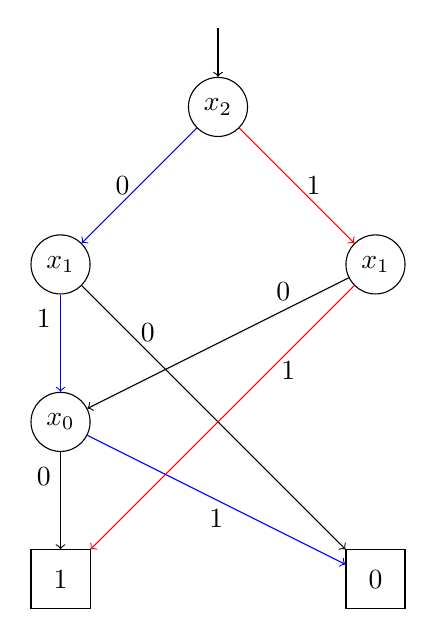
\begin{tikzpicture}[->]
		\tikzstyle{state} = [circle,draw,minimum size=0.75cm]
		\tikzstyle{final}  = [rectangle,draw,shape aspect=1,minimum size=0.75cm]
		
		\node[state] (x2) at (20,20) {$x_2$};
		\node[state] (x10) at (18,18) {$x_1$};
		\node[state] (x11) at (22,18) {$x_1$};
		\node[state] (x0) at (18,16) {$x_0$};
		\node[final] (f1) at (18,14) {$1$};
		\node[final] (f0) at (22,14) {$0$};
		
		\path (20,21) edge (x2);
		\path (x2) edge[blue] node[black,left] {0} (x10);
		\path (x2) edge[red] node[black,right] {1} (x11);
		
		\path (x10) edge[blue] node[black,left,near start] {1} (x0);
		\path (x10) edge[black] node[black,above,near start] {0} (f0);
		
		\path (x11) edge[black] node[black,above,near start] {0} (x0);
		\path (x11) edge[red] node[black,below,near start] {1} (f1);
		
		\path (x0) edge[black] node[black,left,near start] {0} (f1);
		\path (x0) edge[blue] node[black,below] {1} (f0);
	\end{tikzpicture}
	\caption{BDD highlighting boolean variable assignment $x_2x_1x_0 = 011$ in blue and $x_2x_1 = 11$ in red}
	\label{fig:ex_simplebdd}
\end{figure}
	
	The path created from variable assignment $x_2x_1x_0 = 011$ is highlighted in blue in the diagram and shows that this assignment is indeed not satisfied by the boolean formula. The red path shows the variable assignments $110$ and $111$. Determining the path and the outcome for every variable assignment results in the same truth table as seen in Example \ref{ex_boolform}.
\end{example}

Given $n$ boolean variables and two boolean functions encoded as BDDs we can perform binary operations $\vee,\wedge$ on the BDDs in $O(N_a * N_b)$, where $N_a$ and $N_b$ are the number of nodes in the decision diagrams of the two functions. A decision diagram is a tree with $n$ levels, so $N_a = O(2^n)$ and $N_b = O(2^n)$. Therefore with $n$ boolean variables we can perform binary operations $\vee$ and $\wedge$ on them in $O(2^{2n})=O(m^2)$ where $m = 2^n$ is the maximum set size that can be represented by $n$ variables \cite{BDD_running_time,Handbook_BDD_Chapter}. Since the running time specifically depends on the size of the decision diagrams, in general if the boolean functions are simple then the size of the decision diagram is also small and operations can be performed quickly.

\section{Unified parity games}
\label{sec_unified_pg}
We can consider a VPG as a PG that is the union of all its projections. We call the resulting PG the \textit{unification} of the VPG.
\begin{definition}
Given VPG $\hat{G} = (\hat{V},\hat{V}_0,\hat{V}_1, \hat{E},\hat{\Omega}, \mathfrak{C},\theta)$ we define the unification of $\hat{G}$, denoted as $\hat{G}_{\downarrow}$, as
\[  \hat{G}_{\downarrow} = \bigcup_{c\in \mathfrak{C}}\hat{G}_{|c} \]
where the union of two PGs is trivially defined as
\[ (V,V_0,V_1,E,\Omega) \cup (V',V_0',V_1',E',\Omega') = (V \cup V', V_0 \cup V_0', V_1 \cup V_1', E \cup E', \Omega \cup \Omega') \]
\end{definition}
We will use the hat decoration ($\hat{G},\hat{V},\hat{E},\hat{\Omega},\hat{W}$) when referring to a VPG and use no hat decoration when referring to a PG.

Every vertex in game $\hat{G}_{\downarrow}$ originates from a configuration and an original vertex. Therefore we can consider every vertex in a unification as a pair consisting of a vertex and a configuration, ie. $V = \mathfrak{C} \times \hat{V}$. We can consider edges in a unification similarly, ie. $E \subseteq (\mathfrak{C} \times \hat{V}) \times (\mathfrak{C} \times \hat{V})$. Note that edges don't cross configurations, ie. for every $((c,\hat{v}) , (c',\hat{v}')) \in E$ we have $c = c'$.

If we solve the PG that is the unification of a VPG we have solved the VPG, as shown in the next theorem .
\begin{theorem}
	\label{theA_solve_UVPG_is_solve_VPG}
	Given VPG $\hat{G} =  (\hat{V},\hat{V}_0,\hat{V}_1, \hat{E},\hat{\Omega}, \mathfrak{C},\theta)$. For winning sets $W_0$ and $W_1$ for game $\hat{G}_{\downarrow}$ and winning sets $\hat{W}^c_0$ and $\hat{W}^c_1$ for some configuration $c \in \mathfrak{C}$ it holds that
	\[(c,\hat{v}) \in W_\alpha \iff \hat{v} \in \hat{W}^c_\alpha  \text{, for }\alpha \in \{0,1\}  \]
	\begin{proof}
		The bi-implication is equal to  the following to implications.
		\[ (c,\hat{v}) \in W_\alpha \implies \hat{v} \in \hat{W}^c_\alpha  \text{, for }\alpha \in \{0,1\} \]
		and
		\[ (c,\hat{v}) \notin W_\alpha\implies \hat{v} \notin \hat{W}^c_\alpha \text{, for }\alpha \in \{0,1\}  \]
		
		Since the winning sets partition the game we have $\hat{v} \notin \hat{W}^c_\alpha \implies \hat{v} \in \hat{W}^c_{\overline{\alpha}}$ (similar for set $W$). Therefore it is sufficient to prove the first implication.
		
		Let $(c,\hat{v}) \in W_\alpha$, player $\alpha$ has a strategy to win game $\hat{G}_{\downarrow}$ from vertex $(c,\hat{v})$. Since $\hat{G}_{\downarrow}$ is the union of all the projections of $\hat{G}$ we can apply the same strategy to game $\hat{G}_{|c}$ to win vertex $\hat{v}$ as player $\alpha$. Because we can win $\hat{v}$ in the projection of $\hat{G}$ to $c$ we have $\hat{v} \in \hat{W}^c_\alpha$.
	\end{proof}
\end{theorem}

One of the properties of a PG is its totality; a game is total if every vertex has at least 1 outgoing vertex. Plays in a total PG will always result in an infinite path. VPGs are total, meaning that every vertex has, for every configuration $c \in \mathfrak{C}$ at least 1 outgoing vertex admitting $c$. Because VPGs are total a unified VPG is also total. For unified VPGs we can however further investigate its totality by introducing the notion of being total for every configuration. 
\begin{definition}
	A unified VPG $(V,V_0,V_1,E,\Omega)$ is total for every configuration iff for every $(c,v) \in V$ there exists a $(c,v') \in V$ such that $((c,v),(c,v')) \in E$.
\end{definition}

It follows that if a unified VPG is total then it is also total for every configuration as shown in the following lemma.
\begin{lemma}
	\label{lem_UVPG_total}
	A unified VPG $G = (V,V_0,V_1,E,\Omega)$ that is total is also total for every configuration.
	\begin{proof}
		Since $G$ is total we have for every $(c,v) \in V$ that there exists a $(c,v') \in V$ such that $((c,v),(c',v')) \in E$. Because unified VPGs don't have edges cross configurations we find that $c = c'$ and therefore $G$ is total for every configuration.
	\end{proof}
\end{lemma}

\subsubsection{Representing unified variability parity games}
Unified VPGs have a specific structure because they are the union of parity games that have the same vertices with the same owner and priority.

We can represent a set $X \subseteq (\mathfrak{C} \times \hat{V})$ as a complete function $f : \hat{V} \rightarrow 2^\mathfrak{C}$. The set $X$ and function $f$ are equivalent, denoted by the operator $=_\lambda$, iff the following relation holds:
\[ (c,\hat{v}) \in X \iff c \in f(\hat{v}) \]
We can also represent edges as a complete function $f : \hat{E} \rightarrow 2^\mathfrak{C}$. The set $E$ and function $f$ are equivalent, denoted by the operator $=_\lambda$, iff the following relation holds:
\[ ((c,\hat{v}),(c,\hat{v}')) \in E \iff c \in f(\hat{v},\hat{v}') \]
We write $\lambda^\emptyset$ to denote the function that maps every element to $\emptyset$, clearly $\lambda^\emptyset =_\lambda \emptyset$. We call using a set of pairs to represent vertices a \textit{set-wise} representation and using functions to represent vertices a \textit{function-wise} representation.


Finally we can simplify the priority function of a unified VPG, we don't actually need to create a new function that is the unification of all the projections, we can simply use the original priority assignment function because the following relation holds:
\[ \hat{\Omega}(c,\hat{v}) = \Omega(\hat{v}) \]

\section{Recursive algorithm}
We can use Zielonka's recursive algorithm to solve VPGs, to do so we will first consider a method of creating a parity game from a VPG, called \textit{unification}.
\subsection{Unified parity games}
We can create a PG from a VPG by taking all the projections of the VPG, which are PGs, and combining them into one PG by taking the union of them. We call the resulting PG the \textit{unification} of the VPG. A parity game that is the result of a unification is called a \textit{unified PG}, also any total subgame of it will be called a unified PG. A unified PG always has a VPG from which it originated.
\begin{definition}
	Given VPG $\hat{G} = (\hat{V},\hat{V}_0,\hat{V}_1, \hat{E},\hat{\Omega}, \mathfrak{C},\theta)$ we define the unification of $\hat{G}$, denoted as $\hat{G}_{\downarrow}$, as
	\[  \hat{G}_{\downarrow} = \biguplus_{c\in \mathfrak{C}}\hat{G}_{|c} \]
	where the union of two PGs is defined as
	\[ (V,V_0,V_1,E,\Omega) \uplus (V',V_0',V_1',E',\Omega') = (V \uplus V', V_0 \uplus V_0', V_1 \uplus V_1', E \uplus E', \Omega \uplus \Omega') \]
\end{definition}
We will use the hat decoration ($\hat{G},\hat{V},\hat{E},\hat{\Omega},\hat{W}$) when referring to a VPG and use no hat decoration when referring to a PG.

Every vertex in game $\hat{G}_{\downarrow}$ originates from a configuration and an original vertex. Therefore we can consider every vertex in a unification as a pair consisting of a vertex and a configuration, ie. $V = \mathfrak{C} \times \hat{V}$. We can consider edges in a unification similarly, so $E \subseteq (\mathfrak{C} \times \hat{V}) \times (\mathfrak{C} \times \hat{V})$. Note that edges don't cross configurations so for every $((c,\hat{v}) , (c',\hat{v}')) \in E$ we have $c = c'$. Figure \ref{fig:VPG2UPG} shows an example of a unification.

\begin{figure}[h]
	\centering
	\begin{subfigure}{1\textwidth}
		\centering
		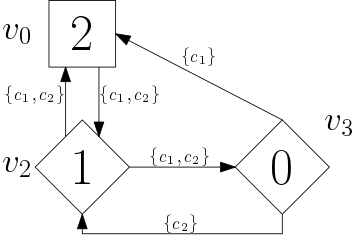
\includegraphics[scale=0.4]{Examples/UPG/VPG}
		\caption{VPG consisting of 2 configurations}
	\end{subfigure}\\
	\begin{subfigure}{1\textwidth}
		\centering
		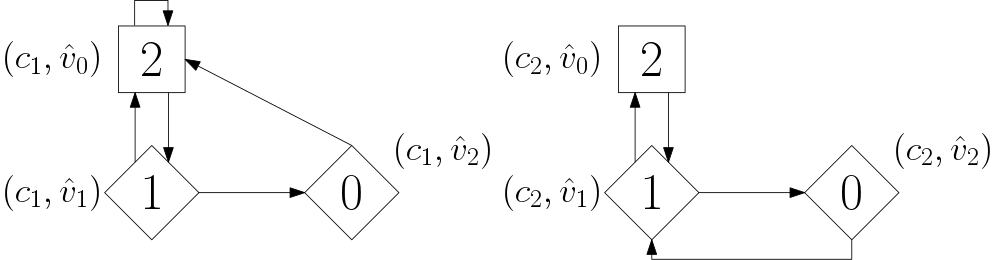
\includegraphics[scale=0.4]{Examples/UPG/UPG}
		\caption{Unified PG, created from unifying the two projections}
	\end{subfigure}
	\caption{A VPG with its corresponding unified PG}
	\label{fig:VPG2UPG}
\end{figure}

If we solve the PG that is the unification of a VPG we have solved the VPG, as shown in the next theorem.
\begin{theorem}
	\label{theA_solve_UVPG_is_solve_VPG}
	Given 
	\begin{itemize}
		\item VPG $\hat{G} =  (\hat{V},\hat{V}_0,\hat{V}_1, \hat{E},\hat{\Omega}, \mathfrak{C},\theta)$,
		\item some configuration $c \in \mathfrak{C}$,
		\item winning sets $\hat{W}^c_0$ and $\hat{W}^c_1$ for game $\hat{G}$ and
		\item winning sets $W_0$ and $W_1$ for game $\hat{G}_{\downarrow}$
	\end{itemize}
	it holds that
	\[(c,\hat{v}) \in W_\alpha \iff \hat{v} \in \hat{W}^c_\alpha  \text{, for }\alpha \in \{0,1\}  \]
	\begin{proof}
		The bi-implication is equal to  the following to implications.
		\[ (c,\hat{v}) \in W_\alpha \implies \hat{v} \in \hat{W}^c_\alpha  \text{, for }\alpha \in \{0,1\} \]
		and
		\[ (c,\hat{v}) \notin W_\alpha\implies \hat{v} \notin \hat{W}^c_\alpha \text{, for }\alpha \in \{0,1\}  \]
		
		Since the winning sets partition the game we have $\hat{v} \notin \hat{W}^c_\alpha \implies \hat{v} \in \hat{W}^c_{\overline{\alpha}}$ (similar for set $W$). Therefore it is sufficient to prove only the first implication.
		
		Let $(c,\hat{v}) \in W_\alpha$, player $\alpha$ has a strategy to win game $\hat{G}_{\downarrow}$ from vertex $(c,\hat{v})$. Since $\hat{G}_{\downarrow}$ is the union of all the projections of $\hat{G}$ we can apply the same strategy to game $\hat{G}_{|c}$ to win vertex $\hat{v}$ as player $\alpha$. Because we can win $\hat{v}$ in the projection of $\hat{G}$ to $c$ we have $\hat{v} \in \hat{W}^c_\alpha$.
	\end{proof}
\end{theorem}

\subsubsection{Projections and totality}
A unified PG can be projected back to one of the games from which it is the union.
\begin{definition}
	The projection of unified PG $G = (V,V_0, V_1,E,{\Omega})$ to configuration $c$, denoted as $G_{|c}$, is the parity game $(V',{V}_0,{V}_1,E',{\Omega})$ such that $V' = \{ {v}\ |\ (c,{v}) \in V \}$ and $E' = \{ ({v},{w})\ |\ ((c,{v}),(c,{w})) \in E \} $.
\end{definition}

One of the properties of a PG is its totality; a game is total if every vertex has at least 1 outgoing vertex. VPGs are also total, meaning that every vertex has, for every configuration $c \in \mathfrak{C}$, at least 1 outgoing vertex admitting $c$. Because VPGs are total their unifications are also total. Since edges in a unified PG don't cross configurations we can conclude that a unified PG is total iff every projection is total.

\subsection{Solving unified PGs}
We can solve a unified PG using the Zielonka's recursive algorithm. The algorithm revolves around the attractor operation and the creation of subgames. Consider the example presented in figure \ref{fig:VPG2UPG}. Vertices with the highest priority are 
\[ \{(c_1,v_0),(c_2,v_0)\}\]
attracting these for player $0$ gives the set 
\begin{align*}
\{(c_1,v_0),&(c_2,v_0),\\
(c_1,v_1),&(c_2,v_1),\\
 &(c_2,v_2)\}
\end{align*}
The algorithm tries to attract all vertices starting from $v_0$ with any configuration, in this case $v_1$ can be attracted for all configurations, $v_2$ can only be attracted for $c_2$. When edge guards are permissive, ie. they admit many configurations, then there is a good change that vertices can be attracted for multiple configurations at the same time during the algorithm. This is the idea for the family based recursive VPG algorithm we represent next, we will use the recursive algorithm to solve unified parity games such that it tries to attract multiple configurations simultaneously.

\subsection{Representing unified parity games}
In order to create an algorithm based around attracting multiple configurations we need to take a look at how unified parity games can be represented.


Unified PGs have a specific structure because they are the union of PGs that have the same vertices with the same owner and priority. Because they have the same priority we don't actually need to create a new function that is the unification of all the projections, we can simply use the original priority assignment function because the following relation holds:
\[ \Omega(c,\hat{v}) = \hat{\Omega}(\hat{v}) \]
Similarly we can use the original partition sets $\hat{V}_0$ and $\hat{V}_1$ instead of having the new partition $V_0$ and $V_1$ because the following relations holds:
\[ (c,\hat{v}) \in V_0 \iff \hat{v}\in \hat{V}_0 \]
\[ (c,\hat{v}) \in V_1 \iff \hat{v}\in \hat{V}_1 \]
So instead of considering unified PG $(V,V_0,V_1,E,\Omega)$ we will consider $(V,\hat{V}_0,\hat{V}_1,E,\hat{\Omega})$. 

Next we consider how we represent vertices and edges in a unified PG. A set $X \subseteq (\mathfrak{C} \times \hat{V})$ can be represented as a complete function $f : \hat{V} \rightarrow 2^\mathfrak{C}$. The set $X$ and function $f$ are equivalent, denoted by the operator $=_\lambda$, iff the following relation holds:
\[ (c,\hat{v}) \in X \iff c \in f(\hat{v}) \]
We can also represent edges as a complete function $f : \hat{E} \rightarrow 2^\mathfrak{C}$. The set $E$ and function $f$ are equivalent, denoted by the operator $=_\lambda$, iff the following relation holds:
\[ ((c,\hat{v}),(c,\hat{v}')) \in E \iff c \in f(\hat{v},\hat{v}') \]
We write $\lambda^\emptyset$ to denote the function that maps every element to $\emptyset$, clearly $\lambda^\emptyset =_\lambda \emptyset$. We call using a set of pairs to represent vertices and edges a \textit{set-wise} representation and using functions a \textit{function-wise} representation.

\subsection{Algorithms}
Using the recursive algorithm as a basis we can solve a VPG product based, alternatively we can solve it family based using a set-wise presentation or a function-wise presentation. For the function-wise presentation we can either use an explicit or a symbolic representation of sets of configurations. The following diagram shows the different algorithms:
\begin{center}
	\begin{forest}
		[Recursive algorithm, for tree={parent anchor=south, child anchor=north, align=center, s sep=5mm}
		[Product based]
		[Family based
		[Set-wise]
		[Function-wise
		[Explicit]
		[Symbolic]
		]
		]
		]
	\end{forest}
\end{center}

\subsection{Recursive algorithm using a function-wise representation}
We can modify the recursive algorithm to work with the function-wise representation of vertices and edges. Pseudo code for the modified algorithm is presented in algorithm \ref{alg_zlnk_UVPG}.
\begin{algorithm}
	\caption{$\textsc{recursiveUVPG}(\textit{PG } G = (\\
		V : \hat{V} \rightarrow 2^\mathfrak{C},\\
		\hat{V}_0 \subseteq \hat{V},\\
		\hat{V}_1 \subseteq \hat{V},\\
		E : \hat{E} \rightarrow 2^\mathfrak{C},\\
		\hat{\Omega} : \hat{V}\rightarrow \mathbb{N}$}\label{alg_zlnk_UVPG}
	\begin{algorithmic}[1]
		\State $m \gets \min\{ \hat{\Omega}(\hat{v})\ |\ V(\hat{v}) \neq \emptyset \}$
		\State $h \gets \max\{ \hat{\Omega}(\hat{v})\ |\ V(\hat{v}) \neq \emptyset \}$
		\If{$h = m$ or $V = \lambda^\emptyset$}
		\If{$h$ is even or $V = \lambda^\emptyset$}
		\State \Return $(V,\lambda^\emptyset)$
		\Else
		\State \Return $(\lambda^\emptyset, V)$
		\EndIf
		\EndIf
		\State $\alpha \gets 0$ if $h$ is even and $1$ otherwise
		\State $U \gets \lambda^\emptyset$, $U(\hat{v}) \gets V(\hat{v})$ for all $\hat{v}$ with $\hat{\Omega}(\hat{v}) = h$
		\State $A \gets \alpha\textit{-FAttr}(G, U)$
		\State $(W_0', W_1') \gets \textsc{recursiveUVPG}(G \backslash A)$
		\If{$W_{\overline{\alpha}}' =\lambda^\emptyset$}
		\State $W_\alpha \gets A \cup W_\alpha'$
		\State $W_{\overline{\alpha}} \gets \lambda^\emptyset$
		\Else
		\State $B \gets \overline{\alpha}\textit{-FAttr}(G,W_{\overline{\alpha}}')$
		\State $(W_0'', W_1'') \gets \textsc{recursiveUVPG}(G \backslash B)$
		\State $W_\alpha \gets W_\alpha''$
		\State $W_{\overline{\alpha}} \gets W_{\overline{\alpha}}'' \cup B$
		\EndIf
		\State \Return $(W_0, W_1)$
	\end{algorithmic}
\end{algorithm}

We introduce a modified attractor definition to work with the function-wise representation.
\begin{definition}
		\label{def_Uattr}Given unified PG $G = (V, \hat{V}_0,\hat{V}_1,E,\hat{\Omega})$ and a non-empty set $U \subseteq V$, both represented function-wise, we define $\alpha\textit{-FAttr}(G,U)$ such that
	\[U_0 = U \]
	For $i \geq 0$:
	\[
	U_{i+1}(\hat{v}) = U_i(\hat{v}) \cup \begin{cases}
V(\hat{v}) \cap \bigcup_{\hat{v}'} (E(\hat{v},\hat{v}') \cap U_i(\hat{v}')) & \text{if } \hat{v} \in \hat{V_{\alpha}}\\
V(\hat{v}) \cap \bigcap_{\hat{v'}}((\mathfrak{C} \backslash E(\hat{v},\hat{v}')) \cup U_i(\hat{v}') & \text{if }\hat{v} \in  \hat{V_{\overline{\alpha}}} \\
	\end{cases}
	\]
	Finally:
	\[\alpha\textit{-FAttr}(G,U) = \bigcup_{i \geq 0} U_i \]
\end{definition}
We will now prove that the function-wise attractor definition gives a result equal to the original definition.
\begin{lemma}
	\label{lem_attr_equal}
	Given unified PG $G = (\mathcal{V},\hat{V}_0,\hat{V}_1, \mathcal{E}, \hat{\Omega})$ and set $\mathcal{U} \subseteq \mathcal{V}$ the function-wise attractor $\alpha\textit{-FAttr}(G,\mathcal{U})$ is equivalent to the set-wise attractor $\alpha\textit{-Attr}(G,\mathcal{U})$ for any $\alpha \in \{0,1\}$.
	\begin{proof}
		Let $V,E,U$ be the set-wise representation and $V^\lambda,E^\lambda,U^\lambda$ be the function-wise representation of $\mathcal{V},\mathcal{E},\mathcal{U}$ respectively.
		
		The following properties hold by definition:
		\[ (c,\hat{v}) \in V \iff c \in V^\lambda(\hat{v})\]
		\[ (c,\hat{v}) \in U \iff c \in U^\lambda(\hat{v})\]
		\[ ((c,\hat{v}),(c,\hat{v}')) \in E \iff c \in E^\lambda(\hat{v},\hat{v}') \]
		
		Since the attractors are inductively defined and $U_0 =_\lambda U^\lambda_0$ (because $U =_\lambda U^\lambda$) we have to prove that for some $i \geq 0$, with $U_i =_\lambda U^\lambda_i$,  we have $U_{i+1} =_\lambda U^\lambda_{i+1}$, which holds iff:
		\[ (c,\hat{v}) \in U_{i+1} \iff c \in U^\lambda_{i+1}(\hat{v}) \]
		Let $(c,\hat{v}) \in V$ (and therefore $c \in V^\lambda(\hat{v})$), we consider 4 cases.
		\begin{itemize}
			\item Case: $\hat{v} \in \hat{V}_{\alpha}$ and $(c,\hat{v}) \in U_{i+1}$:\\
			To prove: $c \in U^\lambda_{i+1}(\hat{v})$.
			
			If $(c,\hat{v}) \in U_i$ then $c \in U^\lambda_i(\hat{v})$ and therefore $c \in U^\lambda_{i+1}(\hat{v})$. If $(c,\hat{v}) \notin U_i$ then we have $c \notin U^\lambda_i(\hat{v})$.
			
			
			Because $\hat{v} \in \hat{V}_{\alpha}$ and $c \in V^\lambda(\hat{v})$ we get
			\[ U^\lambda_{i+1} =\bigcup_{\hat{v}'} (E^\lambda(\hat{v},\hat{v}') \cap U^\lambda_i(\hat{v}')) \]
			
			There exists an $(c',\hat{v}') \in V$ such that $(c',\hat{v}') \in U_i$ and $((c,\hat{v}),(c',\hat{v}')) \in E$. Because edges don't cross configurations we can conclude that $c' = c$. Due to equivalence we have $c \in U^\lambda_i(\hat{v}')$ and $c \in E^\lambda(\hat{v},\hat{v}')$. If we fill this in in the above formula we can conclude that $c \in U^\lambda_{i+1}(\hat{v})$.
			\item Case: $\hat{v} \in \hat{V}_{\alpha}$ and $(c,\hat{v}) \notin U_{i+1}$:\\
			To prove: $c \notin U^\lambda_{i+1}(\hat{v})$.
			
			
			First we observe that since $(c, \hat{v}) \notin U_{i+1}$ we get $(c, \hat{v}) \notin U_{i}$ and therefore $c \notin U^\lambda_i(\hat{v})$.
			
			Because $\hat{v} \in \hat{V}_{\alpha}$ and $c \in V^\lambda(\hat{v})$ we get
\[ U^\lambda_{i+1} =\bigcup_{\hat{v}'} (E^\lambda(\hat{v},\hat{v}') \cap U^\lambda_i(\hat{v}')) \]
			
			Assume $c \in U^\lambda_{i+1}(\hat{v})$. There must exist a $\hat{v}'$ such that $c \in E^\lambda(\hat{v},\hat{v}')$ and $c \in U^\lambda_i(\hat{v}')$. Due to equivalence we have a vertex $((c,\hat{v}),(c,\hat{v}')) \in E$ and $(c,\hat{v}') \in U_i$. In which case $(c,\hat{v})$ would be attracted and would be in $U_{i+1}$ which is a contradiction.
			\item Case: $\hat{v} \in \hat{V}_{\overline{\alpha}}$ and $(c,\hat{v}) \in U_{i+1}$:\\
			To prove: $c \in U^\lambda_{i+1}(\hat{v})$.
			
			If $(c,\hat{v}) \in U_i$ then $c \in U^\lambda_i(\hat{v})$ and therefore $c \in U^\lambda_{i+1}(\hat{v})$. If $(c,\hat{v}) \notin U_i$ then we have $c \notin U^\lambda_i(\hat{v})$.
			
			Because $\hat{v} \in \hat{V}_{\overline{\alpha}}$ we get
			\[ U^\lambda_{i+1} =V^\lambda(\hat{v}) \cap \bigcap_{\hat{v'}}((\mathfrak{C} \backslash E^\lambda(\hat{v},\hat{v}')) \cup U^\lambda_i(\hat{v}') \]
			
			Assume $c \notin U^\lambda_{i+1}(\hat{v})$. Because $c \in V^\lambda(\hat{v})$ there must exist an $\hat{v}$ such that
			\[ c \notin ((\mathfrak{C} \backslash E^\lambda(\hat{v},\hat{v}')) \text{ and } c \notin U^\lambda_i(\hat{v}') \]
			which is equal to
			\[ c \in E^\lambda(\hat{v},\hat{v}') \text{ and } c \notin U^\lambda_i(\hat{v}') \]
			By equivalence we have $((c,\hat{v}),(c,\hat{v}')) \in E$ and $(c,\hat{v}') \notin U_i$. Which means that $(c,\hat{v})$ will not be attracted and $(c,\hat{v}) \notin U_{i+1}$ which is a contradiction.
			\item Case: $\hat{v} \in \hat{V}_{\overline{\alpha}}$ and $(c,\hat{v}) \notin U_{i+1}$:\\
			To prove: $c \notin U^\lambda_{i+1}(\hat{v})$.
			
			First we observe that since $(c, \hat{v}) \notin U_{i+1}$ we get $(c, \hat{v}) \notin U_{i}$ and therefore $c \notin U^\lambda_i(\hat{v})$.
			
			Because $\hat{v} \in \hat{V}_{\overline{\alpha}}$ we get
			\[ U^\lambda_{i+1} =V^\lambda(\hat{v}) \cap \bigcap_{\hat{v'}}((\mathfrak{C} \backslash E^\lambda(\hat{v},\hat{v}')) \cup U^\lambda_i(\hat{v}') \]
			
			Since $(c,\hat{v})$ is not attracted there must exist a $(c,\hat{v}') \in V$ such that 
			\[ ((c,\hat{v}),(c,\hat{v}')) \in E  \text{ and } (c,\hat{v}') \notin U_i \]
			By equivalence we have 
			\[ c \in E^\lambda(\hat{v},\hat{v}')  \text{ and } c \notin U^\lambda_i(\hat{v}') \]
			Which is equal to
			\[ c \notin (\mathfrak{C} \backslash E^\lambda(\hat{v},\hat{v}'))  \text{ and } c \notin U^\lambda_i(\hat{v}') \]
			From which we conclude
			\[ c \notin ((\mathfrak{C} \backslash E^\lambda(\hat{v},\hat{v}')) \cup U^\lambda_i(\hat{v}'))) \]
			Therefore we have $c \notin U^\lambda_{i+1}(\hat{v})$.
		\end{itemize}
	\end{proof}
\end{lemma}

We also introduce a modified subgame definition to work with the function-wise representation.
\begin{definition}
	\label{def_Usubgame}
	For unified PG $G = (V,\hat{V}_0,\hat{V}_1,E,\hat{\Omega})$, represented function-wise, and set $X \subseteq V$ we define the subgame $G \backslash X = (V',\hat{V}_0,\hat{V}_1,E',\hat{\Omega})$ such that:
	\begin{itemize}
		\item $V'(\hat{v}) = V(\hat{v}) \backslash X(\hat{v})$
		\item $E'(\hat{v},\hat{v}') = E(\hat{v},\hat{v}') \cap V'(\hat{v}) \cap V'(\hat{v}')$
	\end{itemize}
\end{definition}
We will now prove that this new subgame definition gives a result equal to the original subgame definition. Note that when using the original subgame definition for unified PGs we can omit the modification to the partition because, as we have seen, we can use the partitioning from the VPG in the representation of unified PGs.
\begin{lemma}
	\label{lem_subgame_eq}
	Given unified PG $G = (\mathcal{V},\hat{V}_0,\hat{V}_1, \mathcal{E}, \hat{\Omega})$ and set $\mathcal{U} \subseteq \mathcal{V}$ the subgame $G \backslash \mathcal{U} = (\mathcal{V}',\hat{V}_0,\hat{V}_1,\mathcal{E}',\hat{\Omega})$ represented set-wise is equal to the subgame represented function-wise.
	\begin{proof}
		Let $V,V',E,E',U$ be the set-wise and $V^\lambda,{V^\lambda}', E^\lambda, {E^\lambda}', U^\lambda$ the function-wise representations of $\mathcal{V},\mathcal{V}', \mathcal{E}, \mathcal{E}', \mathcal{U}$ respectively. We know $V =_\lambda V^\lambda$, $E =_\lambda E^\lambda$ and $U =_\lambda U^\lambda$. To prove: $V' =_\lambda {V^\lambda}'$ and $E' =_\lambda {E^\lambda}'$.
		
		Let $(c,\hat{v}) \in V$.
		
		If $(c,\hat{v}) \in U$ then $c \in U^\lambda(\hat{v})$, also $(c,\hat{v}) \notin V'$ (by definition \ref{def_org_subgame}) and $c \notin {V^\lambda}'(\hat{v})$ (by definition \ref{def_Usubgame}).
		
		If $(c,\hat{v}) \notin U$ then $c \notin U^\lambda(\hat{v})$, also $(c,\hat{v}) \in V'$ (by definition \ref{def_org_subgame}) and $c \in {V^\lambda}'(\hat{v})$ (by definition \ref{def_Usubgame}).
		
		Let $((c,\hat{v}),(c,\hat{w})) \in E$.
		
		If $(c,\hat{v}) \in U$ then $(c,\hat{v}) \notin V'$ and $c \notin {V^\lambda}'(\hat{v})$ (as shown above). We get $((c,\hat{v}),(c,\hat{w})) \notin V' \times V'$ so $((c,\hat{v}),(c,\hat{w})) \notin E'$ (by definition \ref{def_org_subgame}). Also $c \notin {E^\lambda}'(\hat{v},\hat{w})$ (by definition \ref{def_Usubgame}).
		
		If $(c,\hat{w}) \in U$ then we apply the same logic.
		
		If neither is in $U$ then both are in $V'$ and in $V' \times V'$ and therefore the $((c,\hat{v}),(c,\hat{w})) \in E'$. Also we get $c \in {V^\lambda}'(\hat{v})$ and $c \in {V^\lambda}'(\hat{w})$ so we get $c \in {E^\lambda}'(\hat{v},\hat{w})$ (by definition \ref{def_Usubgame}).
	\end{proof}
\end{lemma}

Next we prove the correctness of the algorithm by showing that the winning sets of the function-wise algorithm are equal to the winning sets of the set-wise algorithm.
\begin{theorem}
	Given unified PG $\mathcal{G} = (\mathcal{V},\hat{V}_0,\hat{V}_1, \mathcal{E}, \hat{\Omega})$ the winning sets resulting from \textsc{recursiveUVPG($\mathcal{G}$)} ran over the function-wise representation of $\mathcal{G}$ is equal to the winning sets resulting from \textsc{RecursivePG($\mathcal{G}$)} ran over the set-wise representation of $\mathcal{G}$.
	\begin{proof}
		Let $G = (V,\hat{V}_0,\hat{V}_1,E,\hat{\Omega})$ be the set-wise representation of $\mathcal{G}$ and $G^\lambda = (V^\lambda, \hat{V}_0, \hat{V}_1, E^\lambda, \hat{\Omega})$ be the function-wise representation of $\mathcal{G}$.
		
		Proof by induction on $\mathcal{G}$.
		
		\textbf{Base} When there are no vertices or only one priority \textsc{RecursiveUVPG($G^\lambda$)} returns $\lambda^\emptyset$ and \textsc{RecursivePG($G$)} returns $\emptyset$, these two results are equal therefore the theorem holds in this case.
		
		\textbf{Step}
		Player $\alpha$ gets the same value in both algorithms since the highest priority is equal for both algorithms.
		
		Let $U = \{(c,\hat{v}) \in V\ |\ \hat{\Omega}(\hat{v}) = h \}$ (as calculated by \textsc{RecursivePG}) and $U^\lambda(\hat{v}) = V^\lambda(\hat{v})$ for all $\hat{v}$ with $\hat{\Omega}(\hat{v}) = h$ (as calculated by \textsc{RecursiveUVPG}). We will show that $U =_\lambda U^\lambda$.
		
		Let $(c,\hat{v}) \in U$ then $\hat{\Omega}(\hat{v}) = h$, therefore $U^\lambda(\hat{v}) = V^\lambda(\hat{v})$. Since $U \subseteq V$ we have $(c,\hat{v}) \in V$ and because the equality between $V$ and $V^\lambda$ we get $c \in V^\lambda(\hat{v})$ and $c \in U^\lambda(\hat{V})$.
		
		Let $c \in U^\lambda(\hat{v})$, since $U^\lambda(\hat{v})$ is not empty we have $\hat{\Omega}(\hat{v}) = h$, furthermore $c \in V^\lambda(\hat{v})$ and therefore $(c,\hat{v}) \in V$. We can conclude that $(c, \hat{v}) \in U$ and $U =_\lambda U^\lambda$.
		
		For the rest of the algorithm it is sufficient to see that attractor sets are equal if the game and input set are equal (as shown in lemma \ref{lem_attr_equal}) and that the created subgames are equal (as shown in lemma \ref{lem_subgame_eq}). Since the subgames are equal we can apply the theorem on it by induction and conclude that the winning sets are also equal.
	\end{proof}
\end{theorem}

We have seen in theorem \ref{theA_solve_UVPG_is_solve_VPG} that solving a unified PG solves the VPG, furthermore the algorithm \textsc{RecursiveUVPG} correctly solves a unified PG therefore we can now conclude that for VPG $\hat{G}$ vertex $\hat{v}$ is won by player $\alpha$ for configuration $c$ iff $c \in W_\alpha(\hat{v})$ with $(W_0,W_1) = \textsc{RecursiveUVPG}(G_{\downarrow})$.

\subsubsection{Function-wise attractor set}
Next we present an algorithm to calculate the function-wise attractor, the pseudo code is presented in algorithm \ref{alg_fattr_alg}. The algorithm considers vertices that are in the attracted set for some configuration, for every such vertex the algorithm tries to attract vertices that are connected by an incoming edge. If a vertex is attracted for some configuration then the incoming edges of that vertex will also be considered. We prove the correctness of the algorithm in the following lemma and theorem.
\begin{algorithm}
	\caption{$\textsc{$\alpha$-FAttractor}(G, A : \hat{V} \rightarrow 2^\mathfrak{C})$}\label{alg_fattr_alg}
	\begin{algorithmic}[1]
		\State Queue $Q \gets \{\hat{v} \in \hat{V} \ |\ A(\hat{v}) \neq \emptyset  \}$
		\While{$Q$ is not empty}
		\State $\hat{v}' \gets Q.pop()$
		\For{$E(\hat{v},\hat{v}') \neq \emptyset$}
			\If{$\hat{v} \in \hat{V}_\alpha$}
				\State $a \gets V(\hat{v}) \cap E(\hat{v},\hat{v}') \cap A(\hat{v}')$
			\Else
				\State $a \gets V(\hat{v})$
				\For{$E(\hat{v},\hat{v}'') \neq \emptyset$}
					\State $a \gets a \cap (\mathfrak{C}\backslash E(\hat{v},\hat{v}'') \cup A(\hat{v}''))$
				\EndFor
			\EndIf
			\If{$a \backslash A(\hat{v}) \neq \emptyset$}
				\State $A(\hat{v}) \gets A(\hat{v}) \cup a$
				\State $Q.push(\hat{v})$
			\EndIf
		\EndFor
		\EndWhile
		\State \Return $A$
	\end{algorithmic}
\end{algorithm}
\begin{lemma}
\label{lem_attr_requires_E}
Vertex $\hat{v}$ and configuration $c$, with $c \in V(\hat{v})$, can only be attracted if there is a vertex $\hat{v}'$ such that $c \in E(\hat{v}, \hat{v}')$ and $c \in U_i(\hat{v}')$.
	\begin{proof}
		We first observe that if $\hat{v} \in \hat{V}_\alpha$ then this property follows immediately from definition the function-wise attractor definition (\ref{def_Uattr}). If $\hat{v} \in \hat{V}_{\overline{\alpha}}$ we note that unified PGs are total and therefore all of their projections are also total. So vertex $\hat{v}$ has at least one outgoing edge for $c$, we have $\hat{w}$ such that $c \in E(\hat{v},\hat{w})$. For $\hat{v}$ with $c$ to be attracted we must have $c \in U_i(\hat{w})$.
	\end{proof}
\end{lemma}
\begin{theorem}
Set $A$ calculated by $\textsc{$\alpha$-FAttractor}(G,U)$ satisfies $A = \alpha\textit{-FAttr}(G,U)$.
	\begin{proof} We will prove two loop invariants over the while loop of the algorithm.
		
		\textbf{IV1}: For every $\hat{w} \in \hat{V}$ and $c \in \mathfrak{C}$ with $c \in A(\hat{w})$ we have $c \in \alpha\textit{-FAttr}(G,U)(\hat{w})$.
		
		\textbf{IV2}: For every $\hat{w} \in \hat{V}$ and $c \in \mathfrak{C}$ that can be attracted to $A$ either $c \in A(\hat{w})$ or there exists a $\hat{w}' \in Q$ such that $c \in E(\hat{w},\hat{w}')$.
		
		\textbf{Base}: Before the loop starts we have $A = U$, therefore IV1 holds. Furthermore all the vertices that are in $A$ for some $c$ are also in $Q$ so IV2 holds.
		
		\textbf{Step}: Consider the beginning of an iteration and assume IV1 and IV2 hold. To prove: IV1 and IV2 hold at the end of the iteration.
		
		Set $A$ only contains vertices with configurations that are in $\alpha\textit{-FAttr}(G,U)$. The set is only updated through lines 5-12 and 14 of the algorithm which reflects the exact definition of the attractor set therefore IV1 holds at the end of the iteration.
		
		Consider $\hat{w} \in \hat{V}$ and $c \in \mathfrak{C}$, we distinguish three cases to prove IV2:
		\begin{itemize}
			\item $\hat{w}$ with $c$ can be attracted by the beginning of the iteration but not by the end.
			
			This case can't happen because $A(\hat{w})$ only increases during the algorithm and the values for $E$ and $V$ are not changed throughout the algorithm.
			\item $\hat{w}$ with $c$ can't be attracted by the beginning of the iteration but can by the end.
			
			For $\hat{w}$ with $c$ to be able to be attracted at the end of the iteration there must be some $\hat{w}'$ with $c$ such that during the iteration $c$ was added to $A(\hat{w}')$ (lemma \ref{lem_attr_requires_E}). Every $\hat{w}'$ for which $A(\hat{w}')$ is updated is added to the queue (lines 13-16). Therefore we have $\hat{w}' \in Q$ with $c \in E(\hat{w},\hat{w}')$ and IV1 holds.
			\item $\hat{w}$ with $c$ can be attracted by the beginning of the iteration and also by the end.
			
			Since IV2 holds at the beginning of the iteration we have either $c \in A(\hat{w})$ or we have some $\hat{w}' \in Q$ such that $c \in E(\hat{w},\hat{w}')$. In the former case IV2 holds trivially by the end of the iteration since $A(\hat{w})$ can only increase. For the latter case we distinguish two scenario's. 
			
			First we consider the scenario where vertex $\hat{v}'$ that is considered during the iteration (line 3 of the algorithm) is $\hat{w}'$. There is a vertex $c \in E(\hat{w},\hat{w}')$ by IV2. Therefore we can conclude that $\hat{w}$ is considered in the for loop starting at line $4$ and will be attracted in lines 5-12 and added to $A(\hat{w})$ in line 14. Therefore IV2 holds by the end of the iteration.
			
			Next we consider the scenario where $\hat{v}' \neq \hat{w}'$. In this case by the end of the iteration $\hat{w}'$ will still be in $Q$ and IV2 holds.
		\end{itemize}
	
	Vertices are only added to the queue when something is added to $A$ (if statement on line 13). This can only finitely often happen because $A(\hat{v})$ can never be larger than $V(\hat{v})$ so we can conclude that the while loop terminates after a finite number of iterations.
	
		When the while loop terminates IV1 and IV2 hold so for every $\hat{w} \in \hat{V}$ and $c \in \mathfrak{C}$ that can be attracted to $A$ we have $c \in A(\hat{w})$. Since we start with $A = U$ we can conclude the soundness of the algorithm. IV1 shows the completeness.
	\end{proof}
\end{theorem}


\subsection{Running time}
We will consider the running time for solving VPG $G = (V,V_0,V_1,E,\Omega,\mathfrak{C},\theta)$ product based and family based using the different types of representations. We will use $n$ to denote the number of vertices, $e$ the number of edges, $c$ the number of configurations and $d$ the number of distinct priorities.

The original algorithm runs in $O(e * n^d)$, if we run $c$ parity games independently we get $O(c * e * n ^d)$. We can also apply the original algorithm to a unified PG (represented set-wise) for a family based approach, in this case we get a parity game with $c*n$ vertices and $c*e$ edges. which gives a running time $O(c*e*(c*n)^d)$. However this running time can be improved by using the property that a unified PG consists of $c$ disconnected graphs as we shown next.

We have introduced three types of family based algorithms: set-wise, function-wise with explicit configuration sets and function-wise with symbolic configuration sets. In all three algorithms the running time of the attractor set is dominant, so we need three things: analyse the running time of the base cases, analyse the running time of the attractor set and analyse the recursion.

\textit{Base cases.} In the base cases the algorithm needs to do two things: find the highest and lowest priority and check if there are no more vertices in the game. For the set-wise variant we find the highest and lowest priorities by iterating all vertices, which takes $O(c*n)$. Checking if there are no more vertices is done in $O(1)$. For the function wise algorithms we can find the highest and lowest priority in $O(n)$ and checking if there are no vertices is also done in $O(n)$ since we have to check $V(\hat{v}) = \emptyset$ for every $\hat{v}$. Note that in a symbolic representation using BDDs we can check if a set is empty in $O(1)$ because the decision diagram contains a single node.

\textit{Attractor sets.} For the set-wise family based approach we can use the attractor calculation from the original algorithm which has a time complexity of $O(e)$, so for a unified PG having $c*e$ edges we have $O(c*e)$.

The function-wise variants use a different attractor algorithm. First we consider the variant where sets of configurations are represented explicitly.

Consider algorithm \ref{alg_fattr_alg}. A vertex will be added to the queue when this vertex is attracted for some configuration, this can only happen $c*n$ times, once for every vertex configuration combination. 

The first for loop considers all the incoming edges of a vertex. When we consider all vertices the for loop will have considered all edges, since we consider every vertex at most $c$ times the for loop will run at most $c*e$ times in total.

The second for loop considers all outgoing edges of a vertex. The vertices that are considered are the vertices that have an edge going to the vertex being considered by the while loop. Since the while loop considers $c*n$ vertices the second for loop runs in total at most $c * n * e$ times. The loop itself performs set operations on the set of configurations which can be done in $O(c)$. This gives a total time complexity for the attractor set of $O(n*c^2*e)$.

For the symbolic representation set operations can be done in $O(c^2)$ so we get a time complexity of $O(n*c^3*e)$.

This gives the following time complexities\\
\begin{center}
	\begin{tabular}{|c|c|c|}
		\hline 
		& Base & Attractor set \\ 
		\hline 
		Set-wise & $O(c*n)$ & $O(c*e)$  \\ 
		\hline 
		Function-wise explicit & $O(n)$ &  $O(n*c^2*e)$ \\ 
		\hline 
		Function-wise symbolic & $O(n)$ &  $O(n* c^3*e)$ \\ 
		\hline 
	\end{tabular} 
\end{center}

\textit{Recursion}. The three algorithms behave the same way with regards to their recursion, so we analyse the running time of the set-wise variant and can derive the time complexity of the others using the result.

The algorithm has two recursions, the first recursion lowers the number of distinct priorities by 1. The second recursion removes at least one edge, however the game is comprised of disjoint projections. We can use this fact use in the analyses. Consider unified PG $G$ and $A$ as specified by the algorithm. Now consider the projection of $G$ to an arbitrary configuration $q$, $G_{|q}$. If $(G\backslash A)_{|q}$ contains a vertex that is won by player $\overline{\alpha}$ then this vertex is removed in the second recursion step. If there is no vertex won by player $\overline{\alpha}$ then the game is won in its entirety and the only vertices won by player $\overline{\alpha}$ are in different projections. We can conclude that for every configuration $q$ the second recursion either removes a vertex or $(G\backslash A)_{|q}$ is entirely won by player $\alpha$. Let $\overline{n}$ denote be the maximum number of vertices that are won by player $\overline{\alpha}$ in game $(G\backslash A)_{|q}$. Since every projection has at most $n$ vertices the value for $\overline{n}$ can be at most $n$. Furthermore since $\overline{n}$ depends on $A$, which depends on the maximum priority, the value $\overline{n}$ gets reset when the top priority is removed in the first recursion. We can now write down the recursion of the algorithm:
\[ T(d,\overline{n}) \leq T(d-1,n) + T(d, \overline{n} - 1) + O(c*e) \]
When $\overline{n} = 0$ we will get $W_{\overline{\alpha}} = \emptyset$ as a result of the first recursion. In such a case there will be only 1 recursion.
\[ T(d,0) \leq T(d-1,n) + O(c*e) \]
Finally we have the base case where there is 1 priority:
\[ T(1, \overline{n}) \leq O(c*n) \]
Expanding the second recursion gives
\begin{align*}
T(d) &\leq (n+1)T(d-1) + (n+1)O(c*e)\\
T(1) &\leq O(c*n)
\end{align*}
We will now prove that $T(d) \leq (n+d)^dO(c*e)$ by induction on $d$.

\textbf{Base} $d=1$: $T(1) \leq O(c*n) \leq O(c*e) \leq (n+1)^1O(c*e)$

\textbf{Step} $d > 1$:
\begin{align*}
T(d) &\leq (n+1)T(d-1) + (n+1)O(c*e)\\
&\leq (n+1)(n+d-1)^{d-1}O(c*e) + (n+1)O(c*e)
\end{align*}
Since $n+1 \leq n+d-1$ we get:
\begin{align*}
T(d) &\leq (n+d-1)(n+d-1)^{d-1}O(c*e) + (n+1)O(c*e)\\
&\leq (n+d-1)^dO(c*e) + (n+1)O(c*e)\\
&\leq ((n+d-1)^d + n + 1)O(c*e)
\end{align*}
Using lemma \ref{lem_md_ineq} we get
\begin{align*}
T(d) &\leq (n+d)^dO(c*e)
\end{align*}
This gives a time complexity of $O(c*e*(n+d)^d) = O(c*e*n^d)$. Note that the base time complexity is subsumed in the recursion by the time complexity of the attractor set. Since the time complexity of the attractor set is higher that the time complexity of the base cases for all three variants of algorithms we can simply fill in the attractor time complexity to get $O(n*c^2*e*n^d)$ for the function-wise explicit algorithm and $O(n*c^3*e*n^d)$ for the function-wise symbolic algorithm.

The different algorithms, including their time complexities, are repeated in the diagram below:\\
\begin{center}
	\begin{forest}
	[Recursive algorithm, for tree={parent anchor=south, child anchor=north, align=center, s sep=5mm}
		[Product based\\$O(c*e*n^d)$ ]
		[Family based
			[Set-wise\\$O(c*e*n^d)$ ]
			[Function-wise
				[Explicit\\$O(n * c^2 * e * n^d)$ ]
				[Symbolic\\$O(n * c^3 * e * n^d)$ ]
			]
		]
	]
	\end{forest}
\end{center}

The function wise time complexities consist of three parts:
\begin{itemize}
	\item the number of edges in the queue during the attractor calculation,
	\item the time complexity of set operations on subsets of $\mathfrak{C}$ and
	\item the number of recursions.
\end{itemize}
The number of vertices in the queue during attracting is at most $c*n$, however this number will only be large if we attract a very small number of configurations at a per time we evaluate an edge. Most likely we will be able to attract many configurations at the same time, especially when the VPG originates from an FTS there is a good change that many edges admit most or all configurations in $\mathfrak{C}$. So when there are many similarities in behaviour between the different configurations in the FTS we will have a low number of vertices in the queue.

The time complexity of set operations is $O(c)$ when using an explicit representation and $O(c^2)$ when using a symbolic one. However, as shown in \cite{BDD_running_time}, a breadth-depth first implementation of BDDs keeps a table of already computed results. This allows us to get already calculated results in sublinear time. In total there are $2^c$ possible sets and therefore $2^{2c}$ possible set combinations and $O(2^c)$ possible set operations that can be computed. However when solving a VPG originating from an FTS there will most likely be a relatively small number of different edge guards, in which case the number of unique sets considered in the algorithm will be small and we can often retrieve a set calculation from the computed table.

We can see that even though the running time of the family based symbolic algorithm is the worse, its actual running time might be good when we are able to attract multiple configurations at the same time and have a small number of different edge guards.

\section{Pessimistic parity games}
Given a VPG with configurations $\mathfrak{C}$ we can try to determine sets $P_0,P_1$ such that the vertices in set $P_\alpha$ are won by player $\alpha \in \{0,1\}$ for any configuration in $\mathfrak{C}$. We can do so by creating a \textit{pessimistic} PG; a pessimistic PG is a parity game created from a VPG for a player $\alpha \in \{0,1\}$ such that the PG allows all edges that player $\overline{\alpha}$ might take but only allows edges for $\alpha$ when that edge admits all the configurations in $\mathfrak{C}$.
\begin{definition}
	\label{def_pess_game}
	Given VPG $G = (V,V_0,V_1,E,\Omega, \mathfrak{C},\theta)$, we can create pessimistic PG $G_{\triangleright\alpha}$ for player $\alpha \in \{0,1\}$. We have	
	\[ G_{\triangleright\alpha} = \{V,V_0,V_1,E',\Omega \} \]
	such that
	\[ E' = \{ (v,w) \in E\ |\ v \in V_{\overline{\alpha}} \vee \theta(v,w) = \mathfrak{C} \} \]
\end{definition}


Note that pessimistic parity games are not necessarily total. A play in a PG that is not total might result in a finite path, in such a case the player that can't make a move looses the play.

When solving a pessimistic PG $G_{\triangleright\alpha}$ we get winning sets $W_0,W_1$, every vertex in $W_\alpha$ is winning for player $\alpha$ in $G$ played for any configuration, as shown in the following theorem.
\begin{theorem}
	\label{the_pess_is_winning_for_all_conf}
	Given:
	\begin{itemize}
		\item VPG $G = (V,V_0,V_1,E,\Omega,\mathfrak{C},\theta)$,
		\item configuration $c \in \mathfrak{C}$,
		\item winning sets $W_0^c, W_1^c$ for game $G$,
		\item player $\alpha \in \{0,1\}$ and
		\item pessimistic PG $G_{\triangleright\alpha}$ with winning sets $P_0$ and $P_1$
	\end{itemize}
we have $P_\alpha \subseteq W_\alpha^c$.
	\begin{proof}
		Player $\alpha$ has a strategy in game $G_{\triangleright\alpha}$ such that vertices in $P_\alpha$ are won. We will show that this strategy can also be applied to game $G_{|c}$ to win the same or more vertices.
		
		First we observe that any edge that is taken by player $\alpha$ in game $G_{\triangleright\alpha}$ can also be taken in game $G_{|c}$ so player $\alpha$ can play the same strategy in game $G_{|c}$.
		
		For player $\overline{\alpha}$ there are possibly edges that can be taken in $G_{\triangleright\alpha}$ but can't be taken in $G_{|c}$, in such a case player $\overline{\alpha}$'s choices are limited in game $G_{|c}$ compared to $G_{\triangleright\alpha}$ so if player $\overline{\alpha}$ can't win a vertex in $G_{\triangleright\alpha}$ then he/she can't win that vertex in $G_{|c}$.
		
		We can conclude that applying the strategy from game $G_{\triangleright\alpha}$ in game $G_{|c}$ for player $\alpha$ wins the same or more vertices.
	\end{proof}
\end{theorem}
Figure \ref{fig:VPG2PPGs} shows an example VPG with corresponding pessimistic games, after solving the pessimistic games we find $P_0 = \{v_2\}$ and $P_1 = \{v_0\}$.
\begin{figure}[h]
	\centering
	\begin{subfigure}{1\textwidth}
		\centering
		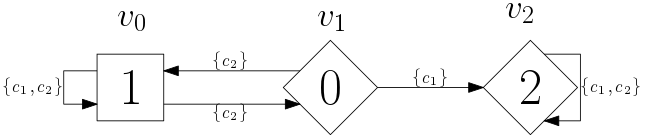
\includegraphics[scale=0.4]{Examples/PPG/VPG}
		\caption{VPG $G$ consisting of 2 configurations}
	\end{subfigure}\\
	\begin{subfigure}{1\textwidth}
		\centering
		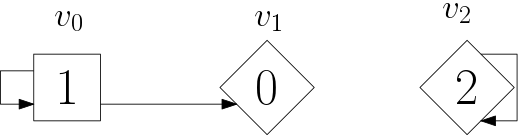
\includegraphics[scale=0.4]{Examples/PPG/P0}
		\caption{Pessimistic game $G_{\triangleright0}$}
	\end{subfigure}\\
	\begin{subfigure}{1\textwidth}
		\centering
		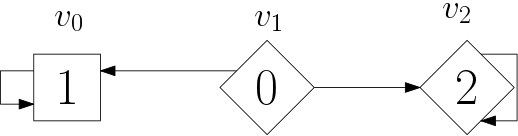
\includegraphics[scale=0.4]{Examples/PPG/P1}
		\caption{Pessimistic game $G_{\triangleright1}$}
	\end{subfigure}
	\caption{A VPG with its corresponding pessimistic games}
	\label{fig:VPG2PPGs}
\end{figure}
\subsection{Configuration partitioning}
We can create a sub-VPG from a VPG by only considering a part of the configurations from the original VPG.
\begin{definition}
	Given VPG $G = (V,V_0,V_1,E,\Omega,\mathfrak{C},\theta)$ and non-empty set $\mathfrak{X} \subseteq \mathfrak{C}$ we define the subgame $G \cap \mathfrak{X} = (V,V_0,V_1,E',\Omega,\mathfrak{C}', \theta')$ such that
	\begin{itemize}
		\item $\mathfrak{C}' =\mathfrak{C} \cap \mathfrak{X}$,
		\item $\theta'(e) = \theta(e) \cap \mathfrak{C}'$ and
		\item $E' = \{ e \in E\ |\ \theta'(e) \neq \emptyset \}$.
	\end{itemize}
\end{definition}
VPGs are total, meaning that for every configuration and every vertex there is an outgoing edge from that vertex admitting that configuration. In subgames the set of configurations is restricted and only edge guards and edges are removed for configurations that fall outside the restricted set, therefore we still have totality.

Furthermore it is trivial to see that every projection $G_{|c}$ is equal to $(G \cap \mathfrak{X})_{|c}$ for any $c \in \mathfrak{C} \cap \mathfrak{X}$.

Finally the subgame operator is associative, meaning $(G \cap \mathfrak{X}) \cap \mathfrak{X}' = G \cap (\mathfrak{X} \cap \mathfrak{X}') = G \cap \mathfrak{X} \cap \mathfrak{X}'$.

Vertices in winning set $P_\alpha$ for $G_{\triangleright\alpha}$ are also winning for player $\alpha$ in pessimistic subgames of $G$, as shown in the following lemma.
\begin{lemma}
	\label{lem_pessimistic_subgames}
	Given:
	\begin{itemize}
		\item VPG $G = (V,V_0,V_1,E,\Omega, \mathfrak{C},\theta)$,
		\item $P_0$ being the winning set of game $G_{\triangleright0}$ for player $0$,
		\item $P_1$ being the winning set of game $G_{\triangleright1}$ for player $1$,
		\item non-empty set $\mathfrak{X} \subseteq \mathfrak{C}$,
		\item player $\alpha \in \{0,1\}$ and
		\item winning sets $Q_0,Q_1$ for game $(G \cap \mathfrak{X})_{\triangleright\alpha}$
	\end{itemize}
	we have
	\[ P_0 \subseteq Q_0 \]
	\[ P_1 \subseteq Q_1 \]
	\begin{proof}
	
		Let edge $(v,w)$ be an edge in game $G_{\triangleright\alpha}$ with $v \in V_\alpha$. Edge $(v,w)$ admits all configuration in $\mathfrak{C}$ so it also admits all configuration in $\mathfrak{C} \cap \mathfrak{X}$, therefore we can conclude that edge $(v,w)$ is also an edge of game $(G\cap \mathfrak{X})_{\triangleright\alpha}$.
		
		Let edge $(v,w)$ be an edge in game $(G \cap \mathfrak{X})_{\triangleright\alpha}$ with $v \in V_{\overline{\alpha}}$. The edge admits some configuration in $\mathfrak{C} \cap \mathfrak{X}$, this configuration is also in $\mathfrak{C}$ so we can conclude that edge $(v,w)$ is also an edge of game $G_{\triangleright\alpha}$.
		
		We have concluded that game $(G \cap \mathfrak{X})_{\triangleright\alpha}$ has the same or more edges for player $\alpha$ as game $G_{\triangleright\alpha}$ and the same or less edges for player $\overline{\alpha}$. Therefore we can conclude that any vertex won by player $\alpha$ in $G_{\triangleright\alpha}$ is also won by $\alpha$ in game $(G \cap \mathfrak{X})_{\triangleright\alpha}$, ie. $P_\alpha \subseteq Q_\alpha$.
		
		
		Let $v \in P_{\overline{\alpha}}$, using theorem \ref{the_pess_is_winning_for_all_conf} we find that $v$ is winning for player $\overline{\alpha}$ in $G_{|c}$ for any $c \in \mathfrak{C}$. Because projections of subgames are the same as projections of the original game we can conclude that $v$ is winning for player $\overline{\alpha}$ in $(G \cap \mathfrak{X})_{|c}$ for any $c \in \mathfrak{C} \cap \mathfrak{X}$.
		
		Assume $v \notin Q_{\overline{\alpha}}$ then $v \in Q_{\alpha}$ and using theorem \ref{the_pess_is_winning_for_all_conf} we find that $v$ is winning for player $\alpha$ in $(G \cap \mathfrak{X})_{|c}$ for any $c \in \mathfrak{C} \cap \mathfrak{X}$. This is a contradiction so we can conclude $v \in Q_{\overline{\alpha}}$ and therefore $P_{\overline{\alpha}} \subseteq Q_{\overline{\alpha}}$.
	\end{proof}
\end{lemma}


\begin{appendices}
\section{Auxiliary theorems and lemma's}
\label{appendix:proves}
\begin{lemma}
	\label{lem_md_ineq}
	For $d,m \in \mathbb{N}$ with $d>1$ and $m \geq 0$ the following inequality holds:
	\[ (m+d-1)^d + m+1 \leq (m+d)^d \]
	\begin{proof}
		We expand the inequality.
		\begin{align*}
		(m+d-1)^d + m + 1 & \leq (m+d)^d\\
		(m+d-1)(m+d-1)^{d-1} + m + 1 & \leq (m+d)(m+d)^{d-1}\\
		m(m+d-1)^{d-1} + d(m+d-1)^{d-1} - (m+d-1)^{d-1} + m + 1 & \leq m(m+d)^{d-1} + d(m+d)^{d-1}
		\end{align*}
		Since $d > 1$ and $m \geq 0$ we can see that the left hand term $m(m+d-1)^{d-1}$ is less or equal to the right hand term $m(m+d)^{d-1}$, similarly the left hand term $d(m+d-1)^{d-1}$ is less or equal to the right hand term $d(m+d)^{d-1}$. Finally the term $(m+d-1)^{d-1} \geq (m+1)^{d-1} \geq m+1$ and therefore $- (m+d-1)^{d-1} + m + 1  \leq 0$. This proves the lemma.
	\end{proof}
\end{lemma}
\end{appendices}

\bibliography{mybib} 
\bibliographystyle{ieeetr}

\end{document}
